\section{Proofs and examples}
\bexa\label{eg:fisher}
In the Gaussian case, data fission can be viewed as a continuous analog of data splitting in terms of the allocation of Fisher information.
\newline $ $
Let $\{X_i\}_{i=1}^n$ be \iid $\distNorm(\theta, \sigma^2)$. Let $X \defas \begin{bmatrix} X_1, \dots, X_n \end{bmatrix}^\top$. Data splitting defines $f(X)$ and $g(X)$ as
\[
f^{\text{split}}(X) = \begin{bmatrix} X_1, \dots, X_{an} \end{bmatrix},\quad
g^{\text{split}}(X) = \begin{bmatrix} X_{an+1}, \dots, X_{n} \end{bmatrix},
\]
for $a\in\left\{\frac{1}{n}, \frac{2}{n}, \dots, 1\right\}$.
Note that
\[
\mcI_{f^{\text{split}}(X)} = an\frac{1}{\sigma^2},\quad
\mcI_{g^{\text{split}}(X)} = (1-a)n\frac{1}{\sigma^2}.
\]
On the other hand, data fission first simulates $\{Z_i\}_{i=1}^n$ distributed as \iid $\distNorm(0, \sigma^2)$ and have, for some fixed $\tau\in(0,\infty)$,
\[
f^{\text{fisson}}(X) = \begin{bmatrix} X_1 + \tau Z_1, \dots, X_n + \tau Z_n \end{bmatrix},\quad
g^{\text{fisson}}(X) = \begin{bmatrix} X_1 - \frac{1}{\tau}Z_1, \dots, X_n - \frac{1}{\tau}Z_n \end{bmatrix}.
\]
Note that for all $i\in\{1,\dots,n\}$, $X_i + \tau Z_i \distas \distNorm\left(\theta, (1+\tau^2)\sigma^2 \right)$, $X_i - \frac{1}{\tau} Z_i \distas \distNorm\left(\theta, (1+\frac{1}{\tau^2})\sigma^2 \right)$, and for each $i$, $X_i + \tau Z_i \indep X_i - \frac{1}{\tau} Z_i$. We then have
\[
\mcI_{f^{\text{fisson}}(X)} = n\frac{1}{(1+\tau^2)\sigma^2},\quad
\mcI_{g^{\text{fisson}}(X)} = n\frac{1}{(1+\frac{1}{\tau^2})\sigma^2}.
\]
By setting $a = \frac{1}{1+\tau^2}$, we have $\mcI_{f^{\text{split}}(X)} = \mcI_{f^{\text{fisson}}(X)}$ and $\mcI_{g^{\text{split}}(X)} = \mcI_{g^{\text{fisson}}(X)}$.
\eexa

\bthm\label{thm:conjugacy}
Suppose that for some $A(\cdot), \phi(\cdot), m(\cdot), \theta_1, \theta_2, H(\cdot, \cdot)$, the density of $X$ is given by
\[
p(x \given \theta_1, \theta_2) = m(x)H(\theta_1, \theta_2)\exp\{ \theta_1^\top \phi(x) - \theta_2^\top A(\phi(x)) \}.
\]
Suppose also that there exists $h(\cdot), T(\cdot), \theta_3$ such that
\[
p(z \given x, \theta_3) = h(z)\exp\{ \phi(x)^\top T(z) - \theta_3^\top A(\phi(x)) \}
\]
is a well-defined distribution. First, draw $Z \distas p(z \given X, \theta_3)$, and let $f(X) \defas Z$ and $g(X) \defas X$. Then, $(f(X), g(X))$ satisfy the data fission property (P2). Specifically, note that $f(X)$ has a known marginal distribution
\[
p(z\given \theta_1, \theta_2, \theta_3) = h(z) \frac{H(\theta_1, \theta_2)}{H(\theta_1 + T(z), \theta_2 + \theta_3)},
\]
while $g(X)$ has a known conditional distribution given $f(X)$, which is
\[
p(x\given z, \theta_1, \theta_2, \theta_3) = p(x \given \theta_1 + T(z), \theta_2 + \theta_3).
\]
\ethm
\bprf
Note that because the density $p(z \given x, \theta_3)$ must integrate to $1$, we can view the function $H(\theta_1, \theta_2)$ as a normalization factor since
\[
H(\theta_1, \theta_2) = \frac{1}{\int_{-\infty}^\infty m(x)\exp\{ \theta_1^\top \phi(x) - \theta_2^\top A(\phi(x)) \} dx}.
\]
Therefore, to compute the marginal density, we have
\[
p(z \given \theta_1, \theta_2, \theta_3) &= 
\int_{-\infty}^\infty m(x)h(z)H(\theta_1, \theta_2)\exp \{ (T(z) + \theta_1)^\top \phi(x) - (\theta_2 + \theta_3)^\top A(\phi(x)) \} dx\\
&= h(z)\frac{H(\theta_1, \theta_2)}{H(\theta_1 + T(z), \theta_2 + \theta_3)}.
\]
Similarly, the computation of the conditional density is straightforward
\[
p(x \given z, \theta_1, \theta_2, \theta_3) &= \frac{m(x)h(z)H(\theta_1, \theta_2)\exp\{(T(z)+\theta_1)^\top \phi(x) - (\theta_2 + \theta_3)^\top A(\phi(x))\}}{h(z)\frac{H(\theta_1, \theta_2)}{H(\theta_1 + T(z), \theta_2+\theta_3)}}\\
&= m(x)H(\theta_1 + T(z), \theta_2 + \theta_3)\exp\{ \phi(x)^\top (\theta_1 + T(z)) - (\theta_2 + \theta_3)^\top A(\phi(x)) \}\\
&= p(x \given \theta_1 + T(z), \theta_2 + \theta_3).
\]
This completes the proof.
\eprf

\bexa\label{eg:continuous}
Suppose $X\distas \distGam(\alpha, \beta)$. Draw $Z \distas \distPoiss(\tau X)$, where $\tau\in(0,\infty)$ is a tuning parameter. Let $f(X) = Z$ and $g(X) = X$.
\newline $ $
By writing
\[
\distGam( x \given \alpha, \beta) = \frac{\beta^\alpha}{\Gamma(\alpha)}\exp\{(\alpha-1)\log x - \beta x \},
\]
where $\distGam(\cdot \given \alpha, \beta)$ denotes the pdf of $\distGam(\alpha, \beta)$, we have that $\theta_2 = \beta, \theta_1 = \alpha-1, \phi(x) = \log x, A(\phi(x)) = \exp(\phi(x)) = \exp(\log x) = x, m(x)=1$. Therefore, $H(\theta_1,\theta_2) = \frac{\theta_2^{(\theta_1+1)}}{\Gamma(\theta_1+1)}$. Now since
\[
\distPoiss(z \given \tau x) &= \frac{1}{z!}\exp\{z \log (\tau x) - \tau x\}\\
&= \frac{1}{z!}\exp\{z \log \tau + z \log x - \tau x\}\\
&= \frac{\tau^z}{z!}\exp\{z \log x - \tau x\},
\]
we have that $h(z) = \frac{\tau^z}{z!}, T(z) = z, \theta_3 = \tau$. Therefore, by \cref{thm:conjugacy},
\[
p(z \given \theta_1,\theta_2,\theta_3) &= \frac{\tau^z}{z!}\frac{\frac{\beta^{\alpha}}{\Gamma(\alpha)}}{\frac{(\beta+\tau)^{\left(\alpha + z\right)}}{\Gamma\left( \alpha + z \right)}}\\
&= \frac{(\alpha+z-1)!}{(\alpha-1)!z!}\left(\frac{\beta}{\beta+\tau}\right)^\alpha\left(\frac{\tau}{\beta+\tau}\right)^z\\
&= \distNB\left(z\given \alpha, \frac{\beta}{\beta+\tau} \right);\\
p(x \given z, \theta_1, \theta_2, \theta_3) 
&= \frac{(\beta+\tau)^{\left( \alpha+z \right)}}{\Gamma\left( \alpha + z \right)}
\exp\left\{ \left( \alpha+z-1 \right)\log(x) - (\beta+\tau)x \right\}\\
&= \distGam\left(x \given \alpha+z, \beta+\tau \right).
\]
\eexa

\bexa\label{eg:discrete}
Suppose $X\distas \distGam(\alpha, \beta)$. Draw $Z=(Z_1,\cdots,Z_B)$ where each element is \iid $Z_i \distas \distPoiss(X)$ and $B\in\{1,2,\dots\}$ is a tuning parameter. Let $f(X) = Z$ and $g(X) = X$.
\newline $ $
By writing
\[
\distGam( x \given \alpha, \beta) = \frac{\beta^\alpha}{\Gamma(\alpha)}\exp\{(\alpha-1)\log x - \beta x \},
\]
where $\distGam(\cdot \given \alpha, \beta)$ denotes the pdf of $\distGam(\alpha, \beta)$, we have that $\theta_2 = \beta, \theta_1 = \alpha-1, \phi(x) = \log x, A(\phi(x)) = \exp(\phi(x)) = \exp(\log x) = x, m(x)=1$. Therefore, $H(\theta_1,\theta_2) = \frac{\theta_2^{(\theta_1+1)}}{\Gamma(\theta_1+1)}$. Now since
\[
\distPoiss(z \given x) &= \prod_{i=1}^B\frac{1}{z_i!}\exp\{z_i \log x - x\}\\
&= \left(\prod_{i=1}^B\frac{1}{z_i!}\right)\exp\left\{ \left(\sum_{i=1}^B z_i\right) \log x - Bx \right\},
\]
we have that $h(z) = \prod_{i=1}^B \frac{1}{z_i!}, T(z) = \sum_{i=1}^B z_i, \theta_3 = B$. Therefore, by \cref{thm:conjugacy}, when $B=1$,
\[
p(z \given \theta_1,\theta_2,\theta_3) &= \frac{1}{z!}\frac{\frac{\beta^{\alpha}}{\Gamma(\alpha)}}{\frac{(\beta+1)^{\left(\alpha + z\right)}}{\Gamma\left( \alpha + z \right)}}\\
&= \frac{(\alpha+z-1)!}{(\alpha-1)!z!}\left(\frac{\beta}{\beta+1}\right)^\alpha\left(\frac{1}{\beta+1}\right)^z\\
&= \distNB\left(z\given \alpha, \frac{\beta}{\beta+1} \right);\\
p(x \given z, \theta_1, \theta_2, \theta_3) 
&= \frac{(\beta+1)^{\left( \alpha+z \right)}}{\Gamma\left( \alpha + z \right)}
\exp\left\{ \left( \alpha+z-1 \right)\log(x) - (\beta+1)x \right\}\\
&= \distGam\left(x \given \alpha+z, \beta+1 \right).
\]
However, when $B>1$,
\[
p(z \given \theta_1,\theta_2,\theta_3) &= \left(\prod_{i=1}^B \frac{1}{z_i!}\right)\frac{\frac{\beta^{\alpha}}{\Gamma(\alpha)}}{\frac{(\beta+B)^{\left(\alpha + \sum_{i=1}^B z_i\right)}}{\Gamma\left( \alpha + \sum_{i=1}^B z_i \right)}}\\
&\neq \prod_{i=1}^B \distNB\left( z_i \given \alpha, \frac{\beta}{\beta+B} \right);\\
p(x \given z, \theta_1, \theta_2, \theta_3) 
&= \frac{(\beta+B)^{\left( \alpha+\sum_{i=1}^B z_i \right)}}{\Gamma\left( \alpha + \sum_{i=1}^B z_i \right)}
\exp\left\{ \left( \alpha-1+\sum_{i=1}^B z_i \right)\log(x) - (\beta+B)x \right\}\\
&= \distGam\left(x \given \alpha+\sum_{i=1}^B z_i, \beta+B \right).
\]
\eexa

%\bexa\label{eg:gam_discrete}
%Assume for all $i \in \{1,2,\dots,n\}$, $Y_i \distiid \distGam(\alpha, \exp(\beta^\top x_i))$, where each $x_i\in\reals^d$ is fixed. Following the data fission procedure in \cref{eg:discrete}, with $B=1$, we have that for all $i$, $f(Y_i) = Z_i, g(Y_i) = Y_i$. In the selection phase of selective inference, for some fixed $\lambda>0$, we can do model selection via the optimization below
%\[
%\hbeta_\lambda &= \argmin_{\beta\in\reals^d} -\sum_{i=1}^n \left(\log \distNB\left(z_i \given \alpha, \frac{\exp(\beta^\top x_i)}{\exp(\beta^\top x_i)+1}  \right)\right) + \lambda\|\beta_1\|\\
%&= \argmin_{\beta\in\reals^d} \left(\sum_{i=1}^n -\log{{z_i + \alpha - 1} \choose z_i } - z_i\log\left( \frac{1}{\exp(\beta^\top x_i)+1} \right) - \alpha\log\left( \frac{\exp(\beta^\top x_i)}{\exp(\beta^\top x_i)+1} \right)\right) + \lambda\|\beta_1\|,
%\]
%which is convex in $\beta$. Denote the index set of nonzero entries in $\hbeta_\lambda$ to be $\mcM$ and $|\mcM| = d' \leq d$.
%\newline $ $
%Using the selected features $\mcM$, with $x_{i,\mcM}$ denoting the selected features for the $i$th observation, we can obtain the estimates $\hbeta_n(\mcM)$ via
%\[
%&\hbeta_n(\mcM) \\
%&= \argmin_{\beta\in\reals^{d'}} - \sum_{i=1}^n \left( \log\distGam(y_i \given \alpha + z_i, \exp(\beta^\top x_{i,\mcM}) + 1) \right)\\
%&= \argmin_{\beta\in\reals^{d'}} \sum_{i=1}^n -(\alpha+z_i)\log\left( \exp(\beta^\top x_{i,\mcM}) + 1 \right) + \log\Gamma(\alpha+z_i) - (\alpha+z_i-1)\log y_i + \left( \exp(\beta^\top x_{i,\mcM}) + 1 \right)y_i,
%\]
%which may be convex in $\beta$ but without an argmin, or non-convex (depending on the value of $\alpha$). Therfore, we can instead use the working model
%\[
%&\hbeta_n(\mcM) \\
%&= \argmin_{\beta\in\reals^{d'}} - \sum_{i=1}^n \left( \log\distGam(y_i \given \alpha + z_i, \exp(\beta^\top x_{i,\mcM}) ) \right)\\
%&= \argmin_{\beta\in\reals^{d'}} \sum_{i=1}^n -(\alpha+z_i)\log\left( \exp(\beta^\top x_{i,\mcM}) \right) + \log\Gamma(\alpha+z_i) - (\alpha+z_i-1)\log y_i + \left( \exp(\beta^\top x_{i,\mcM}) \right)y_i.
%\]
%For this problem, we have that
%\[
%\frac{\partial m_i}{\partial \eta_i} = \exp(\beta^\top x_{i,\mcM}), \quad
%m_i = \frac{\alpha+z_i}{\exp(\beta^\top x_{i,\mcM})}, \quad
%v_i = \frac{\alpha+z_i}{\left(\exp(\beta^\top x_{i,\mcM})\right)^2}.
%\]
%Let $D,V,M, G$ be diagonal matrices with
%\[
%D_{ii} = \frac{\partial m_i}{\partial \eta_i}, \quad
%V_{ii} = v_i, \quad
%M_{ii} = m_i, \quad
%G_{ii} = g(y_i) - m_i,
%\]
%then the plug-in estimator for variance becomes
%\[
%\hat{H}_n^{-1}\hat{V}_n\hat{H}_n^{-1} = \left( X_\mcM^\top D^2V^{-1} X_\mcM \right)^{-1}\left( X_\mcM^\top G^2 V^{-2} D^2 X_\mcM \right)\left( X_\mcM^\top D^2V^{-1} X_\mcM \right)^{-1}.
%\]
%\eexa

\bexa\label{eg:gam_cont}
Assume for all $i \in \{1,2,\dots,n\}$, $Y_i \distiid \distGam(\alpha, \exp(\beta^\top x_i))$, where each $x_i\in\reals^d$ is fixed. Following the data fission procedure in \cref{eg:continuous}, we have that for all $i$, $f(Y_i) = Z_i, g(Y_i) = Y_i$. In the selection phase of selective inference, for some fixed $\lambda>0$, we can do model selection via the optimization below
\[
\hbeta_\lambda &= \argmin_{\beta\in\reals^d} -\sum_{i=1}^n \left(\log \distNB\left(z_i \given \alpha, \frac{\exp(\beta^\top x_i)}{\exp(\beta^\top x_i)+\tau}  \right)\right) + \lambda\|\beta_1\|\\
&= \argmin_{\beta\in\reals^d} \left(\sum_{i=1}^n -\log{{z_i + \alpha - 1} \choose z_i } - z_i\log\left( \frac{1}{\exp(\beta^\top x_i)+\tau} \right) - \alpha\log\left( \frac{\exp(\beta^\top x_i)}{\exp(\beta^\top x_i)+\tau} \right)\right) + \lambda\|\beta_1\|,
\]
which is convex in $\beta$. Denote the index set of nonzero entries in $\hbeta_\lambda$ to be $\mcM$ and $|\mcM| = d' \leq d$.
\newline $ $
Using the selected features $\mcM$, with $x_{i,\mcM}$ denoting the selected features for the $i$th observation, we can obtain the estimates $\hbeta_n(\mcM)$ via
\[
&\hbeta_n(\mcM) \\
&= \argmin_{\beta\in\reals^{d'}} - \sum_{i=1}^n \left( \log\distGam(y_i \given \alpha + z_i, \exp(\beta^\top x_{i,\mcM}) + \tau) \right)\\
&= \argmin_{\beta\in\reals^{d'}} \sum_{i=1}^n -(\alpha+z_i)\log\left( \exp(\beta^\top x_{i,\mcM}) + \tau \right) + \log\Gamma(\alpha+z_i) - (\alpha+z_i-1)\log y_i + \left( \exp(\beta^\top x_{i,\mcM}) + \tau \right)y_i,
\]
which may be convex in $\beta$ but without an argmin, or non-convex (depending on the value of $\alpha$). Therefore, we can instead use an alternative working model
\[
&\hbeta_n(\mcM) \\
&= \argmin_{\beta\in\reals^{d'}} - \sum_{i=1}^n \left( \log\distGam(y_i \given \alpha + z_i, \exp(\beta^\top x_{i,\mcM}) ) \right)\\
&= \argmin_{\beta\in\reals^{d'}} \sum_{i=1}^n -(\alpha+z_i)\log\left( \exp(\beta^\top x_{i,\mcM}) \right) + \log\Gamma(\alpha+z_i) - (\alpha+z_i-1)\log y_i + \left( \exp(\beta^\top x_{i,\mcM}) \right)y_i.
\]
For this problem, we have that
\[
\frac{\partial m_i}{\partial \eta_i} = \exp(\beta^\top x_{i,\mcM}), \quad
m_i = \frac{\alpha+z_i}{\exp(\beta^\top x_{i,\mcM})}, \quad
v_i = \frac{\alpha+z_i}{\left(\exp(\beta^\top x_{i,\mcM})\right)^2}.
\]
Let $D,V,M, G$ be diagonal matrices with
\[
D_{ii} = \frac{\partial m_i}{\partial \eta_i}, \quad
V_{ii} = v_i, \quad
M_{ii} = m_i, \quad
G_{ii} = g(y_i) - m_i.
\]
Following the procedure in Appendix A.5 in \cite{leiner2022data}, we have the following plug-in estimator for variance
\[
\hat{H}_n^{-1}\hat{V}_n\hat{H}_n^{-1} = \left( X_\mcM^\top D^2V^{-1} X_\mcM \right)^{-1}\left( X_\mcM^\top G^2 V^{-2} D^2 X_\mcM \right)\left( X_\mcM^\top D^2V^{-1} X_\mcM \right)^{-1}.
\]
We can then construct confidence intervals with significance level $\alpha$, for $k\in\{1,\dots,p\}$ by
\[
[\hbeta_n]_k \pm z_{\frac{\alpha}{2}} \sqrt{[\hat{H}_n^{-1}\hat{V}_n\hat{H}_n^{-1}]_{kk}}.
\]
Note now the quality of this confidence interval depends on the robustness of the working model.
\eexa

\section{Additional simulation details}\label{apdx:plots}
\begin{table}[H]
\centering
\caption{Number of runs that do not select any variable}
\label{tab:num_none}
\begin{tabular}{ccccc}
                  & n=10  & n=20 & n=50 & n=100 \\
                  \hline\\
Data splitting    & 103 & 60 & 1  & 0   \\
Data fission (P1) & 72  & 49 & 0  & 0   \\
Data fission (P2) & 66  & 41 & 0  & 0  
\end{tabular}
\end{table}

\captionsetup[subfigure]{labelformat=empty}
\begin{figure}[ht!]
\centering
\begin{subfigure}[b]{.40\columnwidth} 
    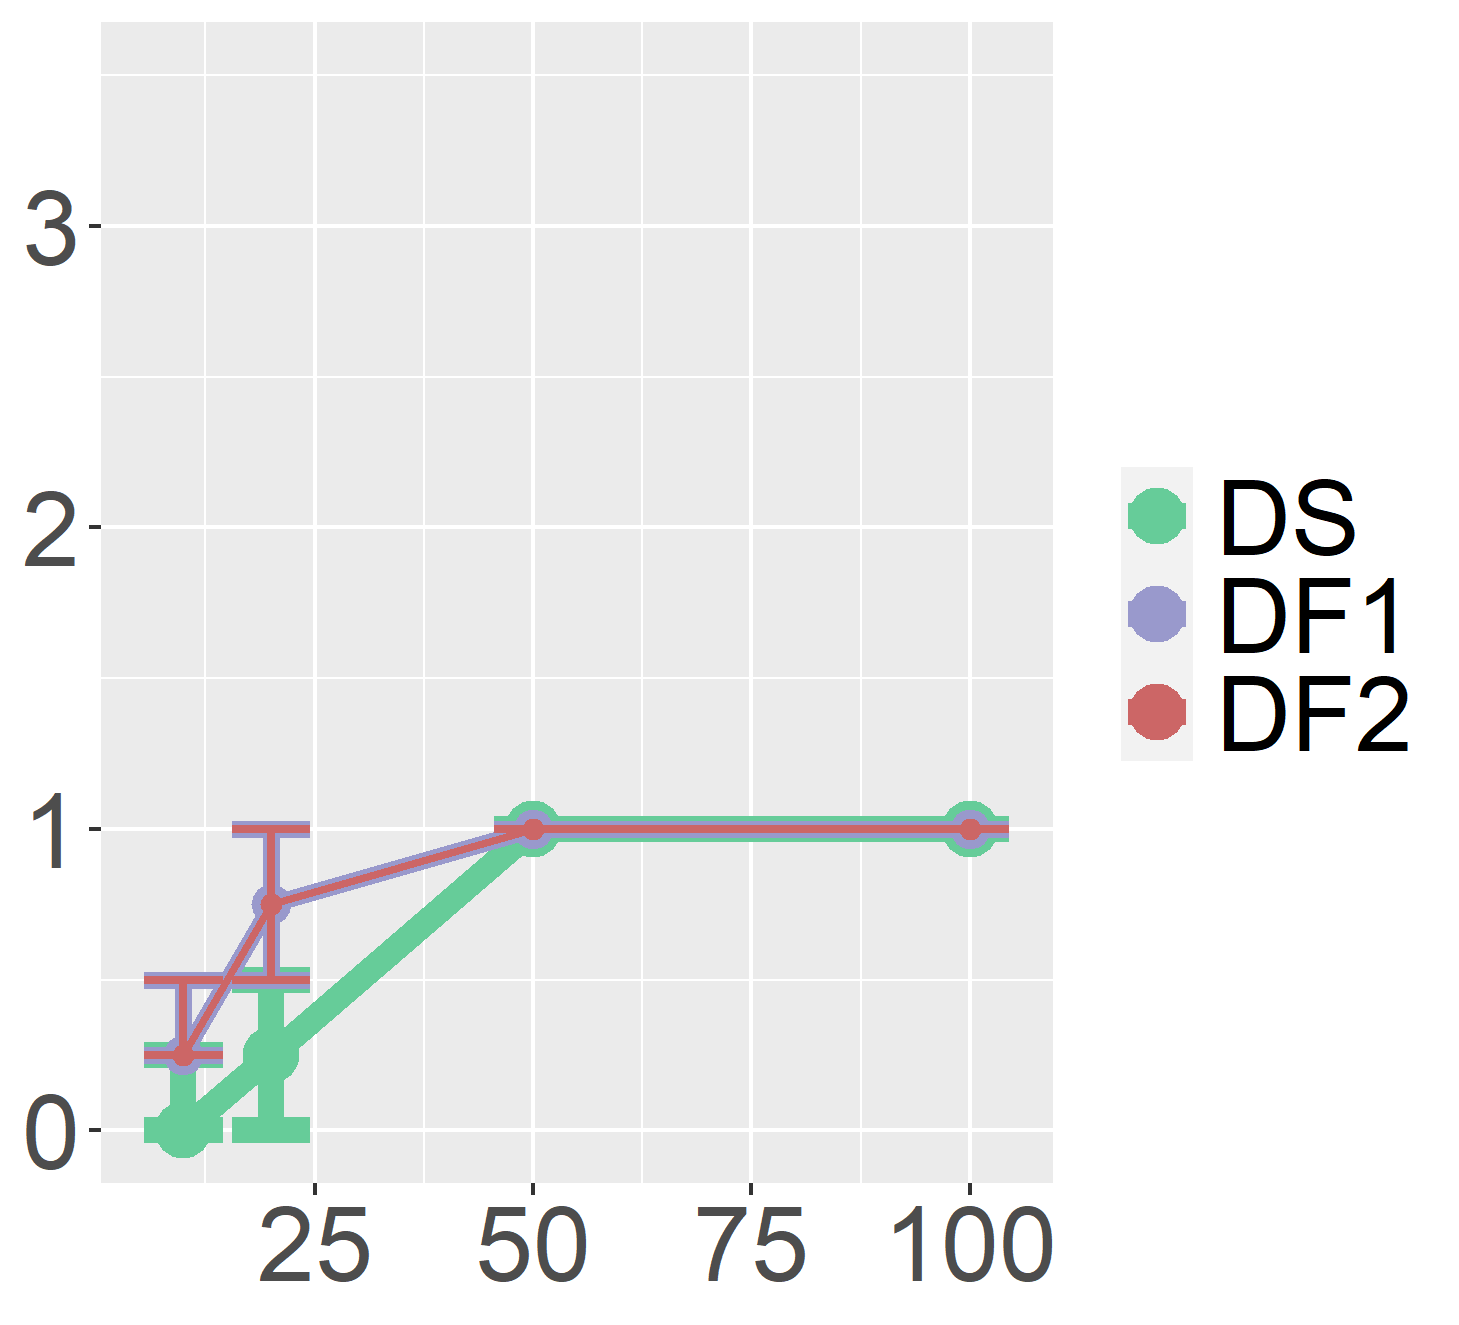
\includegraphics[width=\columnwidth]{../../plot/power_1_IQR.png}
    \caption{(a) Power}
\end{subfigure}
\hfill
\centering
\begin{subfigure}[b]{.40\columnwidth} 
    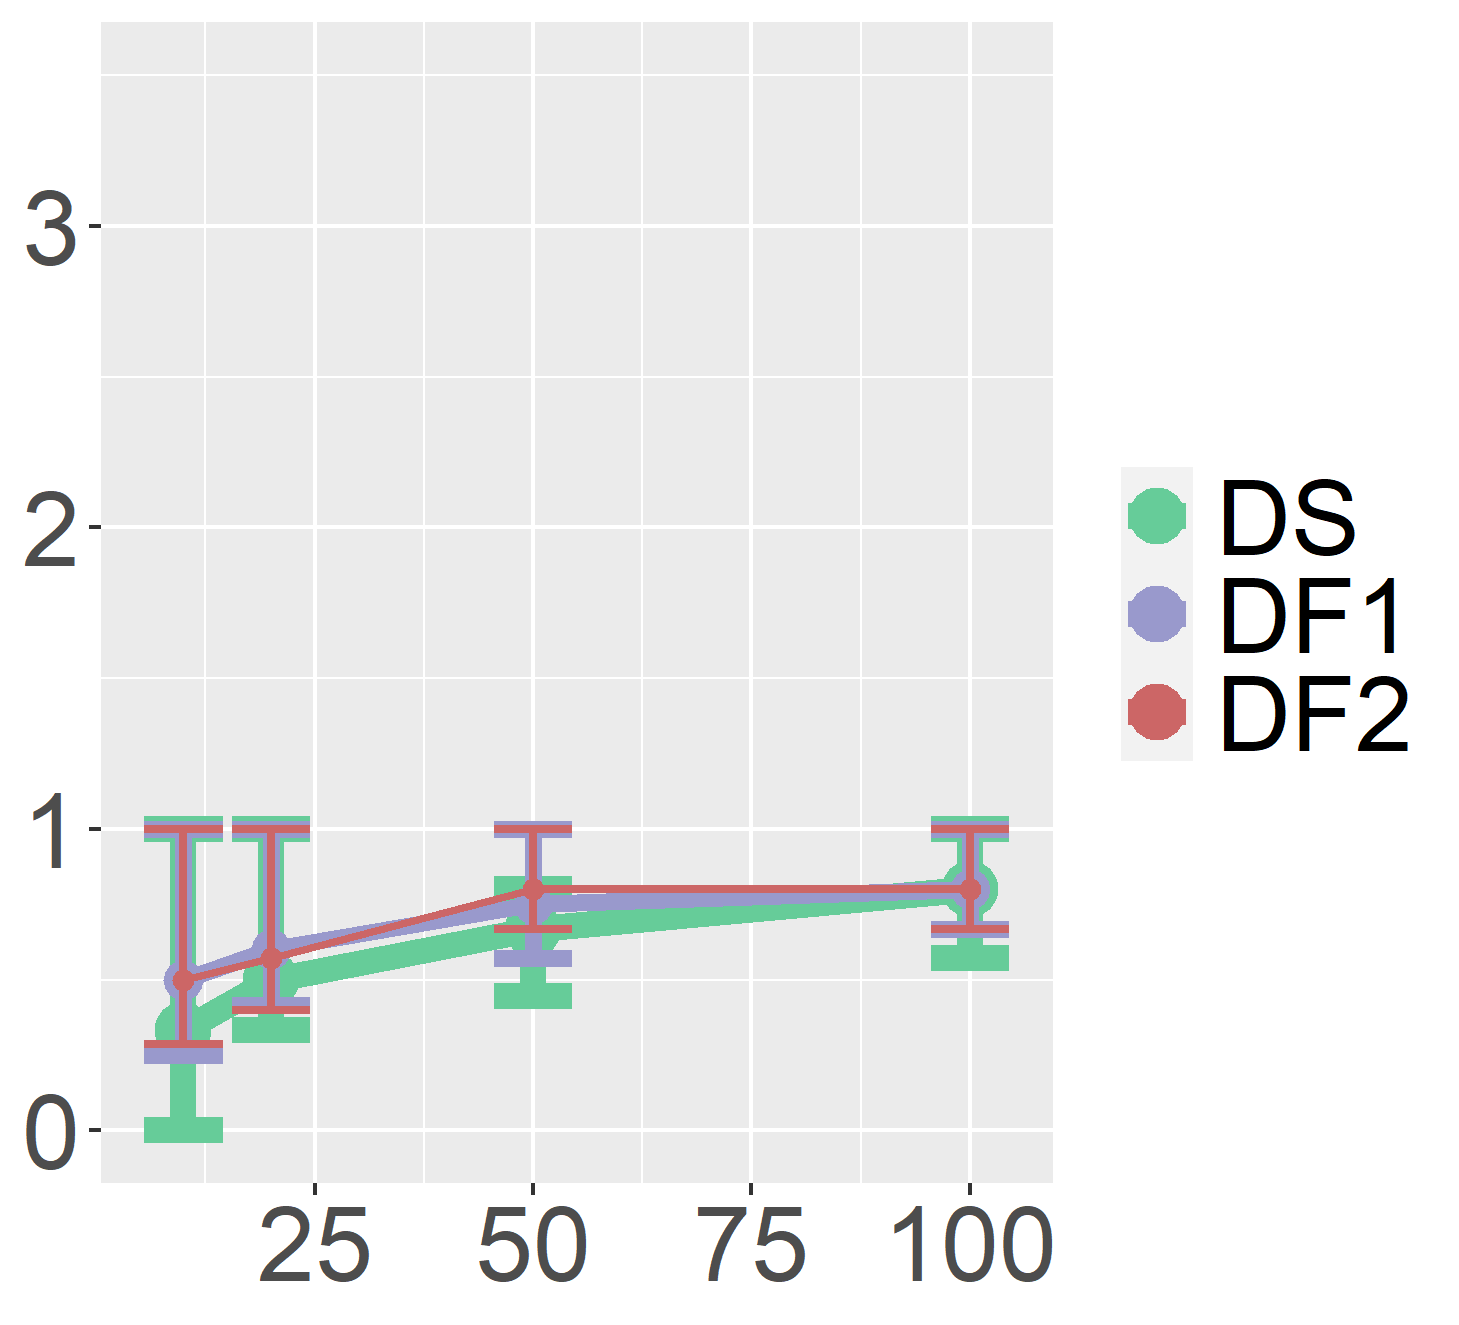
\includegraphics[width=\columnwidth]{../../plot/precision_1_IQR.png}
    \caption{(b) Precision}
\end{subfigure}
\\
\centering
\begin{subfigure}[b]{.40\columnwidth} 
    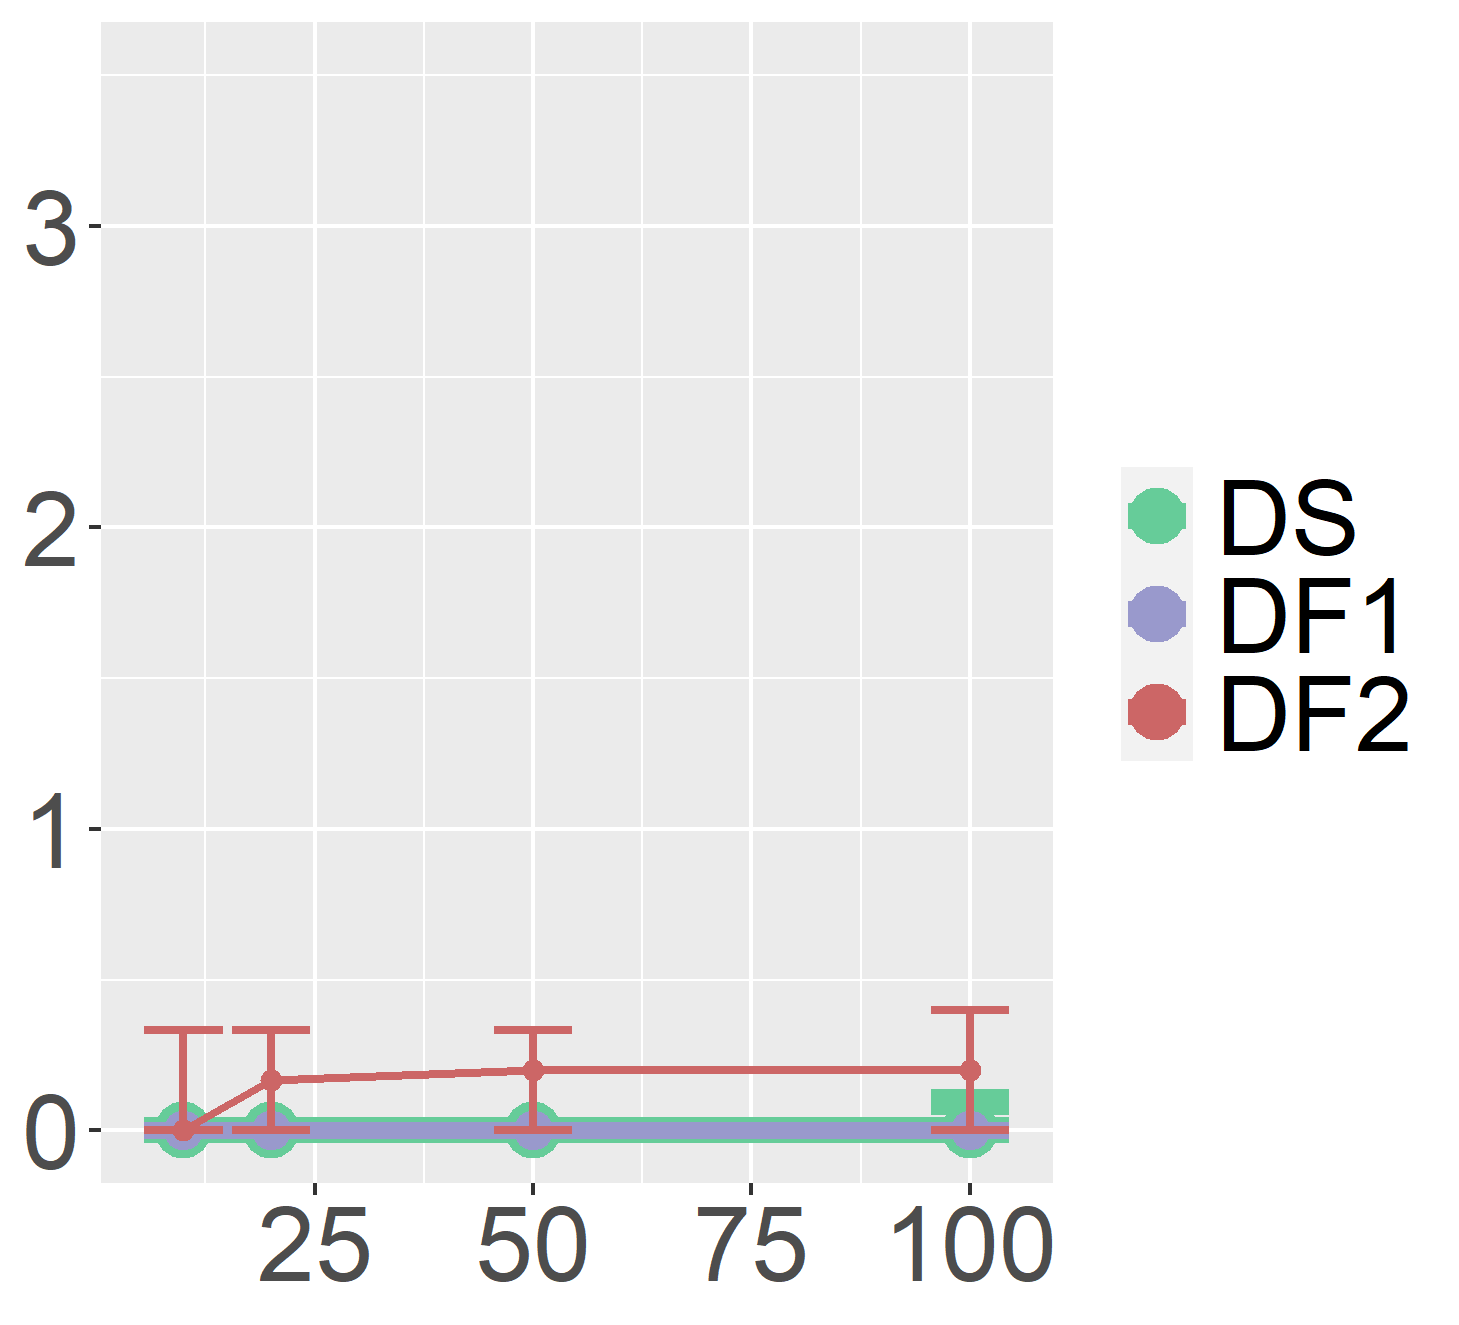
\includegraphics[width=\columnwidth]{../../plot/FCR_1_IQR.png}
    \caption{(c) FCR}
\end{subfigure}
\hfill
\centering
\begin{subfigure}[b]{.40\columnwidth} 
    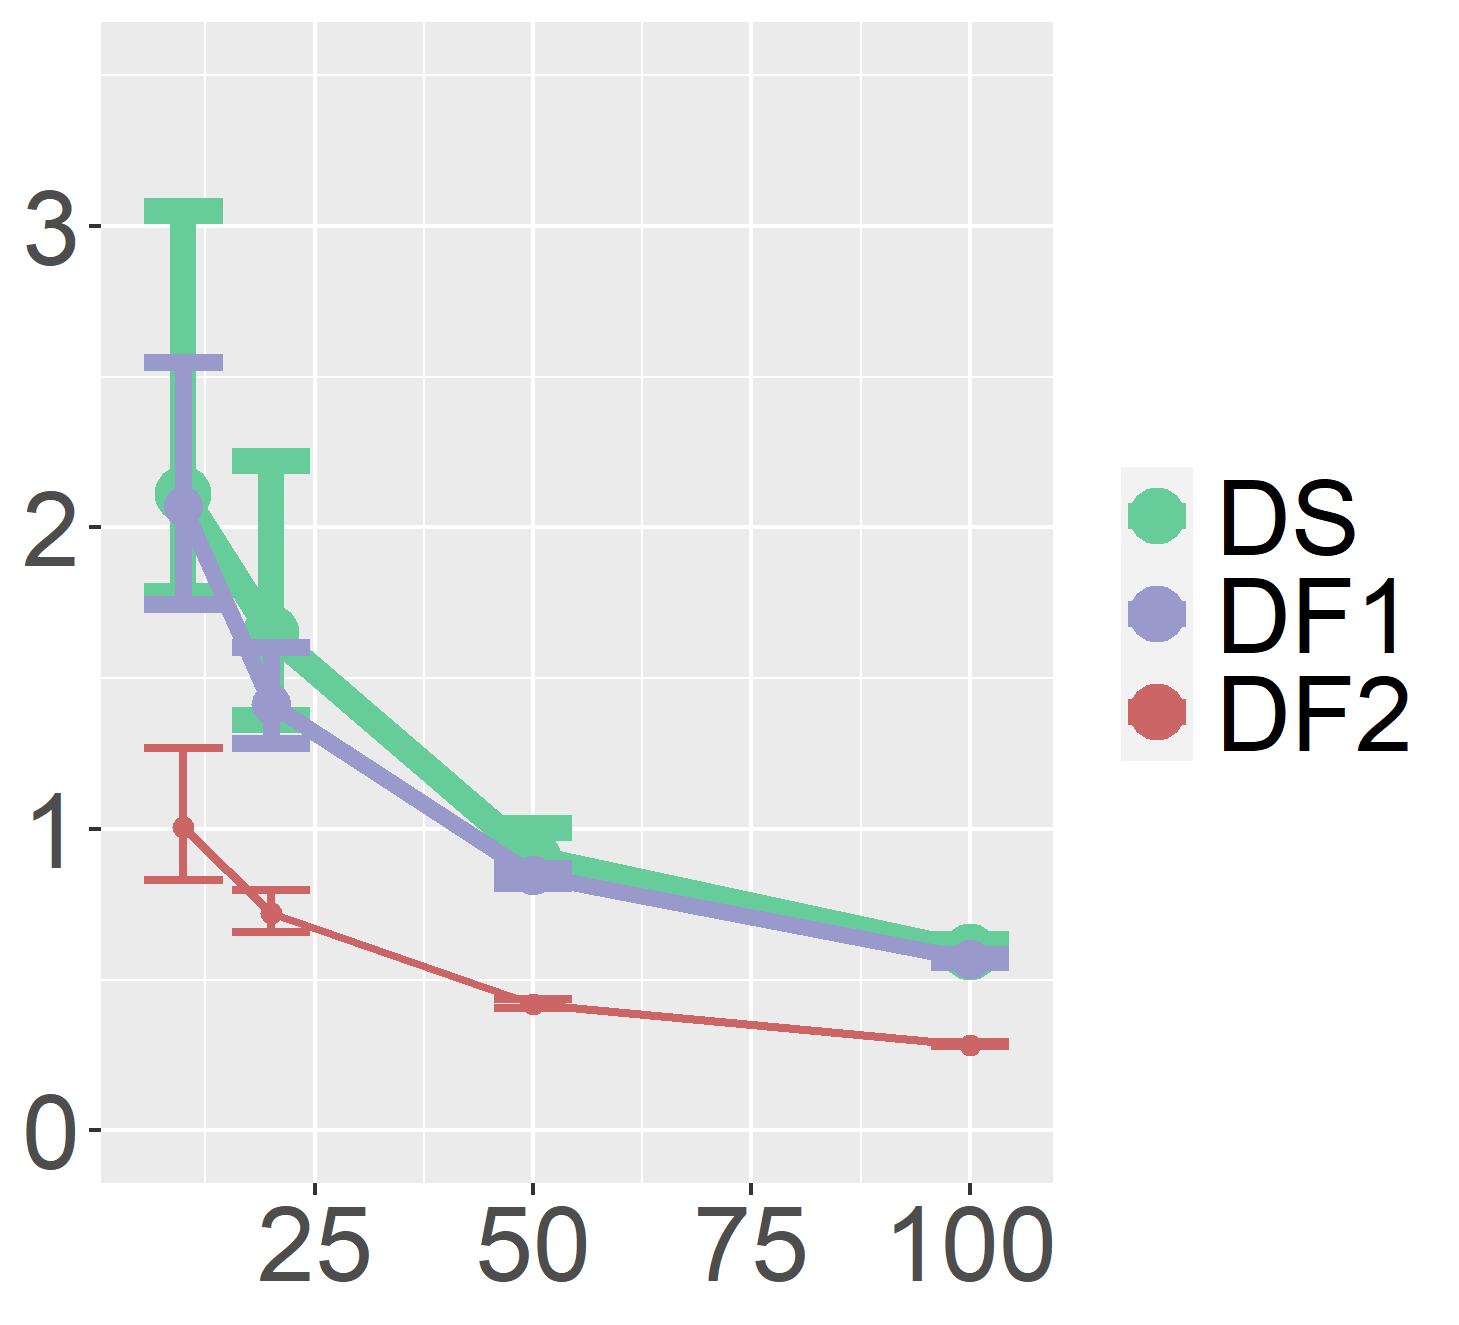
\includegraphics[width=\columnwidth]{../../plot/len_1_IQR.png}
    \caption{(d) Average CI length}
\end{subfigure}
\\
\centering
\begin{subfigure}[b]{.40\columnwidth} 
    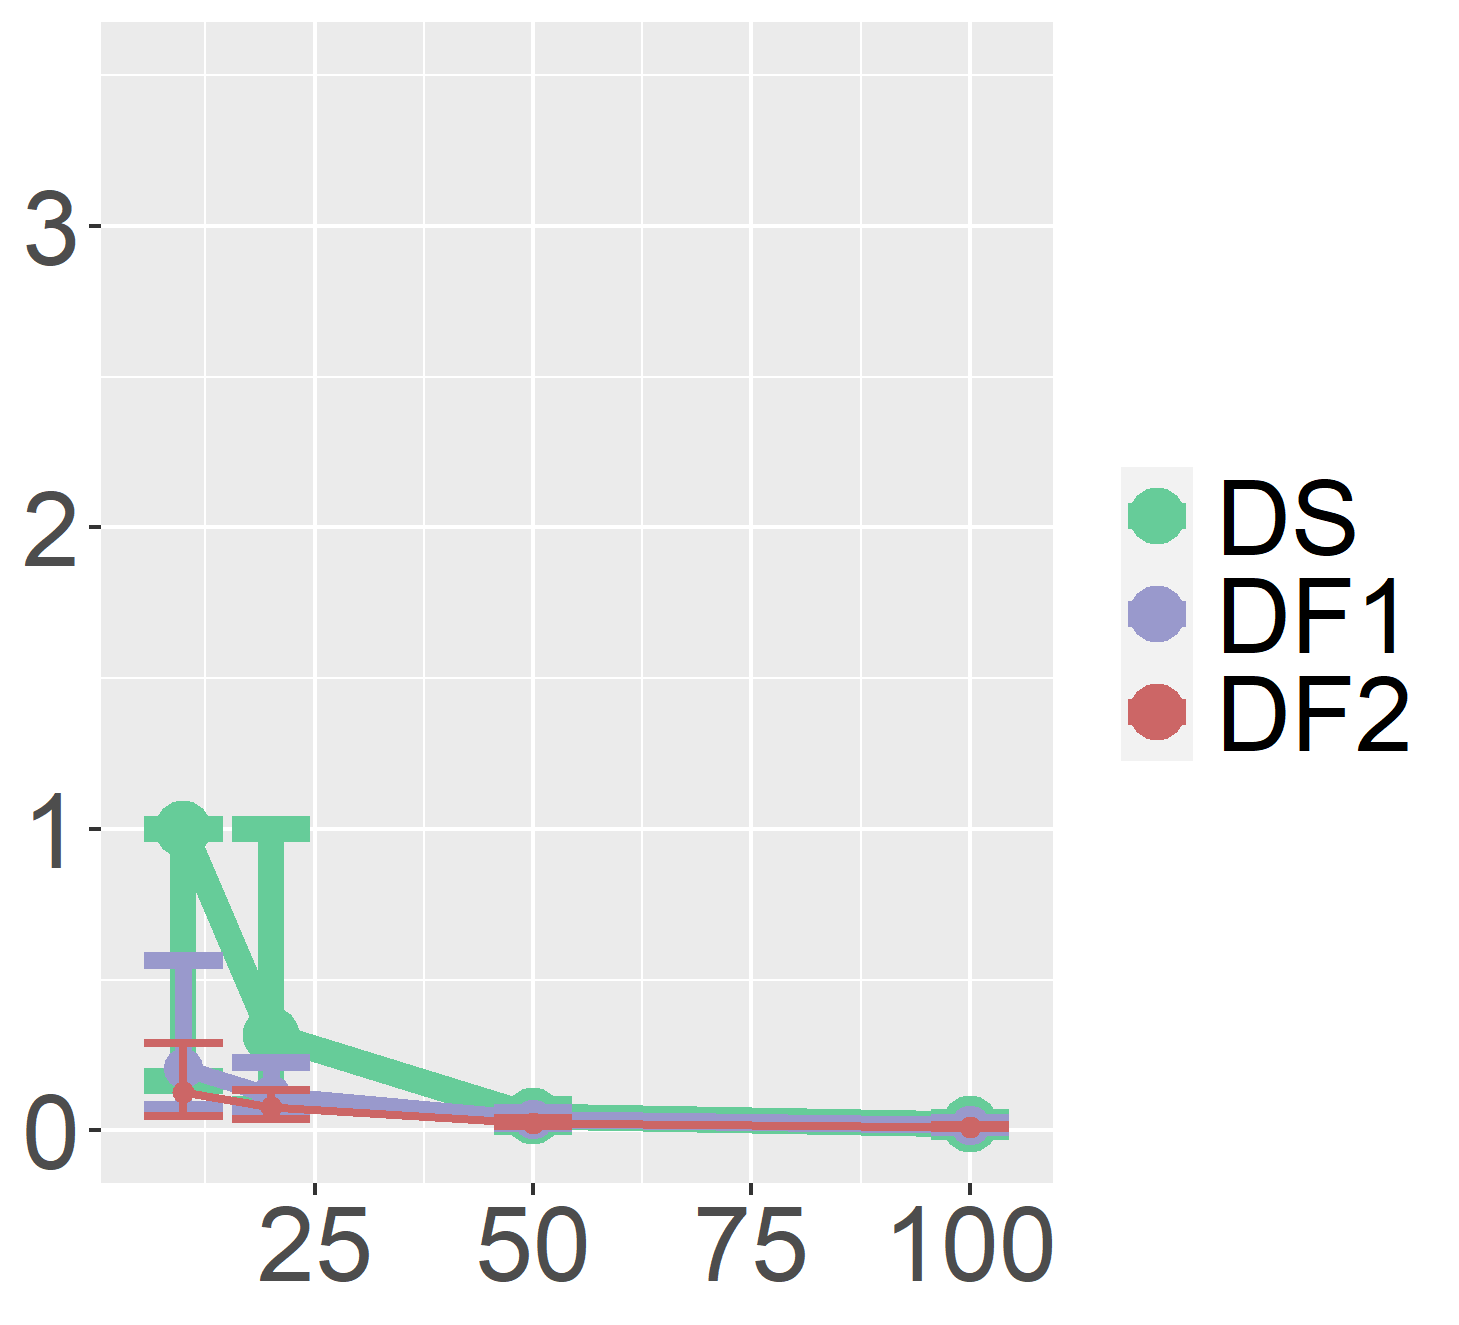
\includegraphics[width=\columnwidth]{../../plot/L2_1_IQR.png}
    \caption{(e) L2 error}
\end{subfigure}
\hfill
\caption{refer to table to explain large IQR when sample size small}
\label{fig:IQR}
\end{figure}

\captionsetup[subfigure]{labelformat=empty}
\begin{figure}[ht!]
\centering
\begin{subfigure}[b]{.32\columnwidth} 
    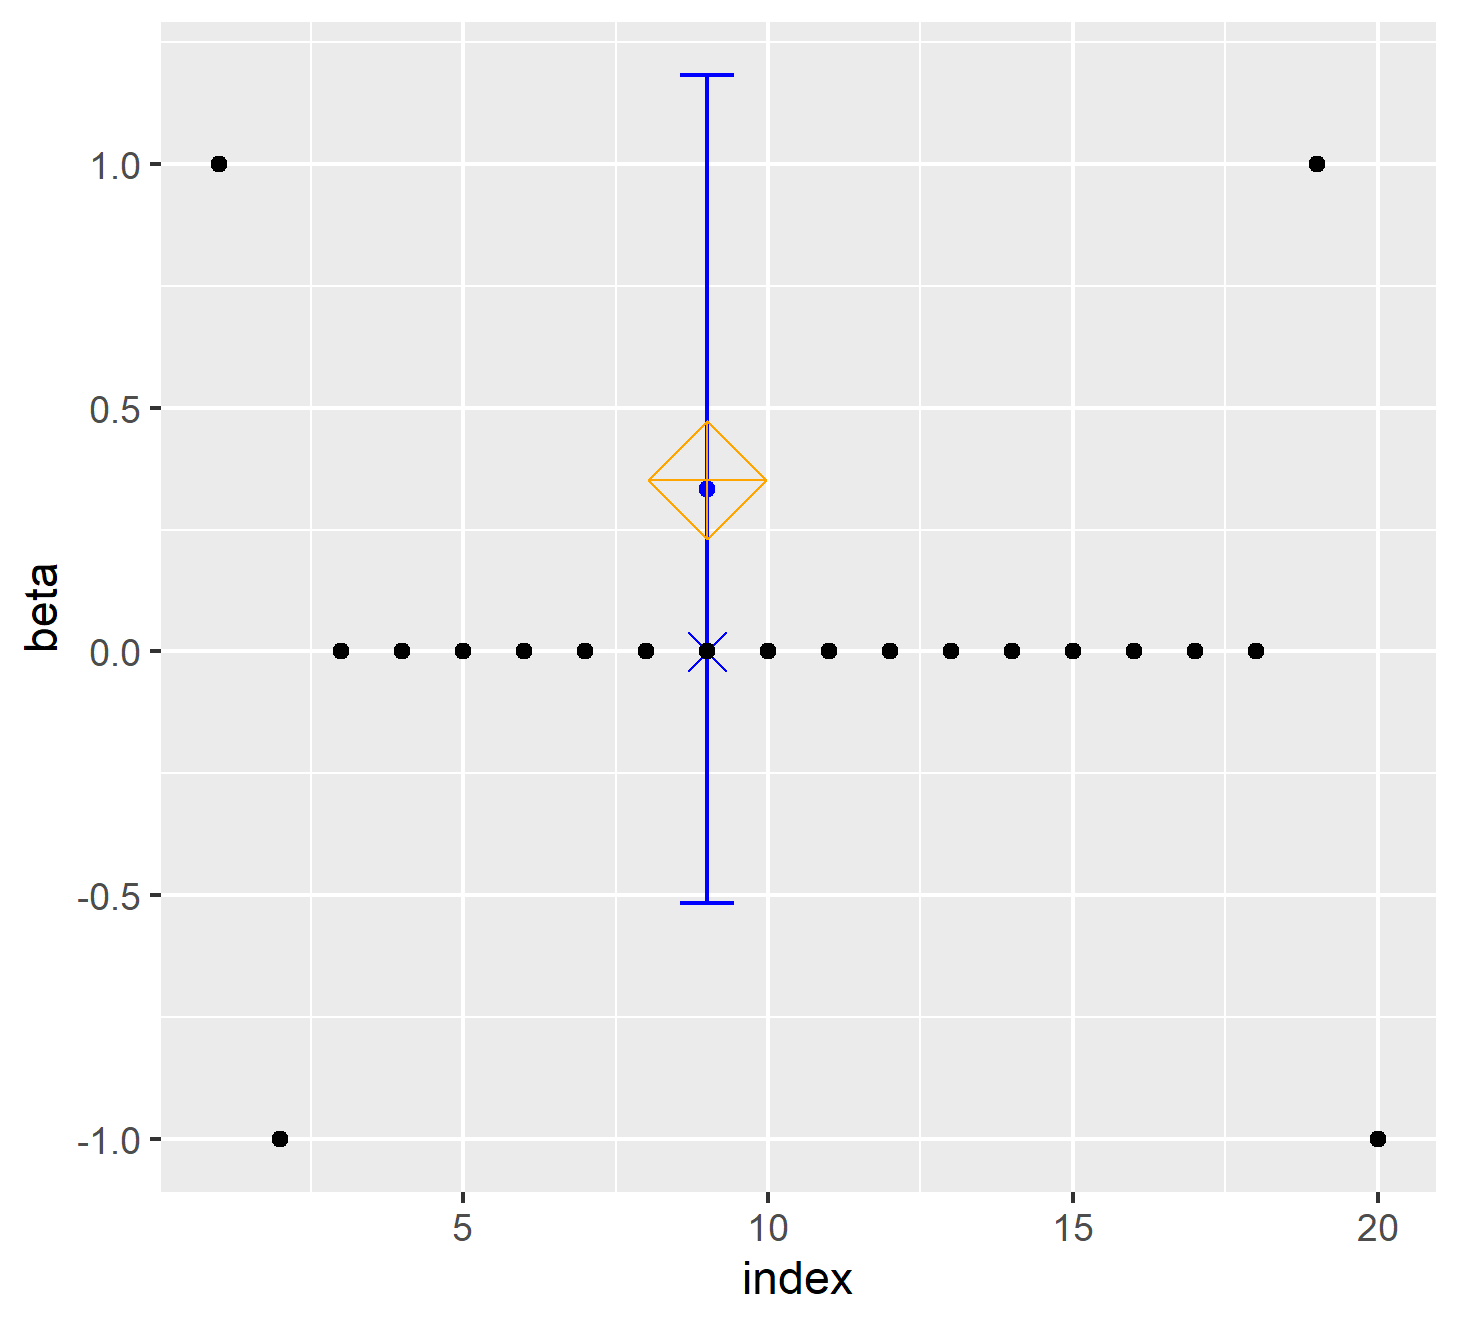
\includegraphics[width=\columnwidth]{../../plot/split_10_1_1.png}
    \caption{(a) Data splitting $n=10$}
    \label{fig:split10}
\end{subfigure}
\hfill
\centering
\begin{subfigure}[b]{.32\columnwidth} 
    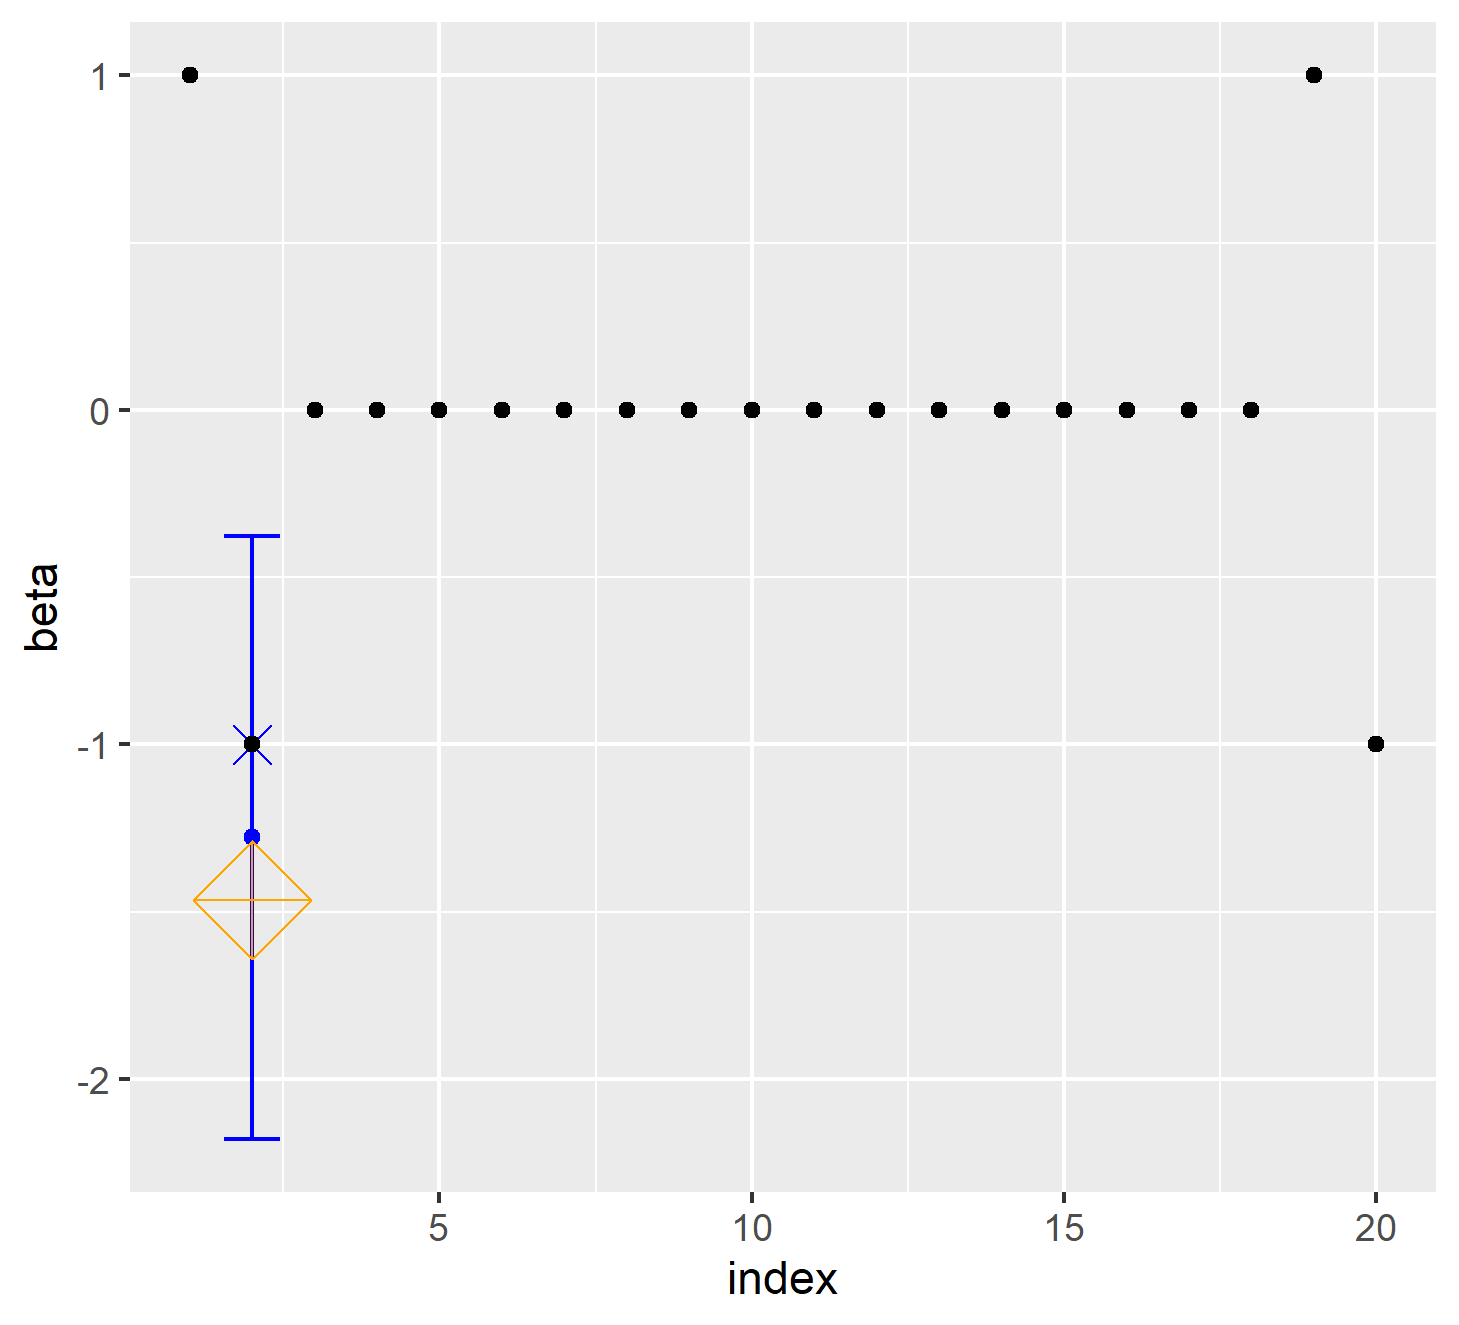
\includegraphics[width=\columnwidth]{../../plot/p1_10_1_1.png}
    \caption{(b) Data fission (P1) $n=10$}
\end{subfigure}
\hfill
\centering
\begin{subfigure}[b]{.32\columnwidth} 
    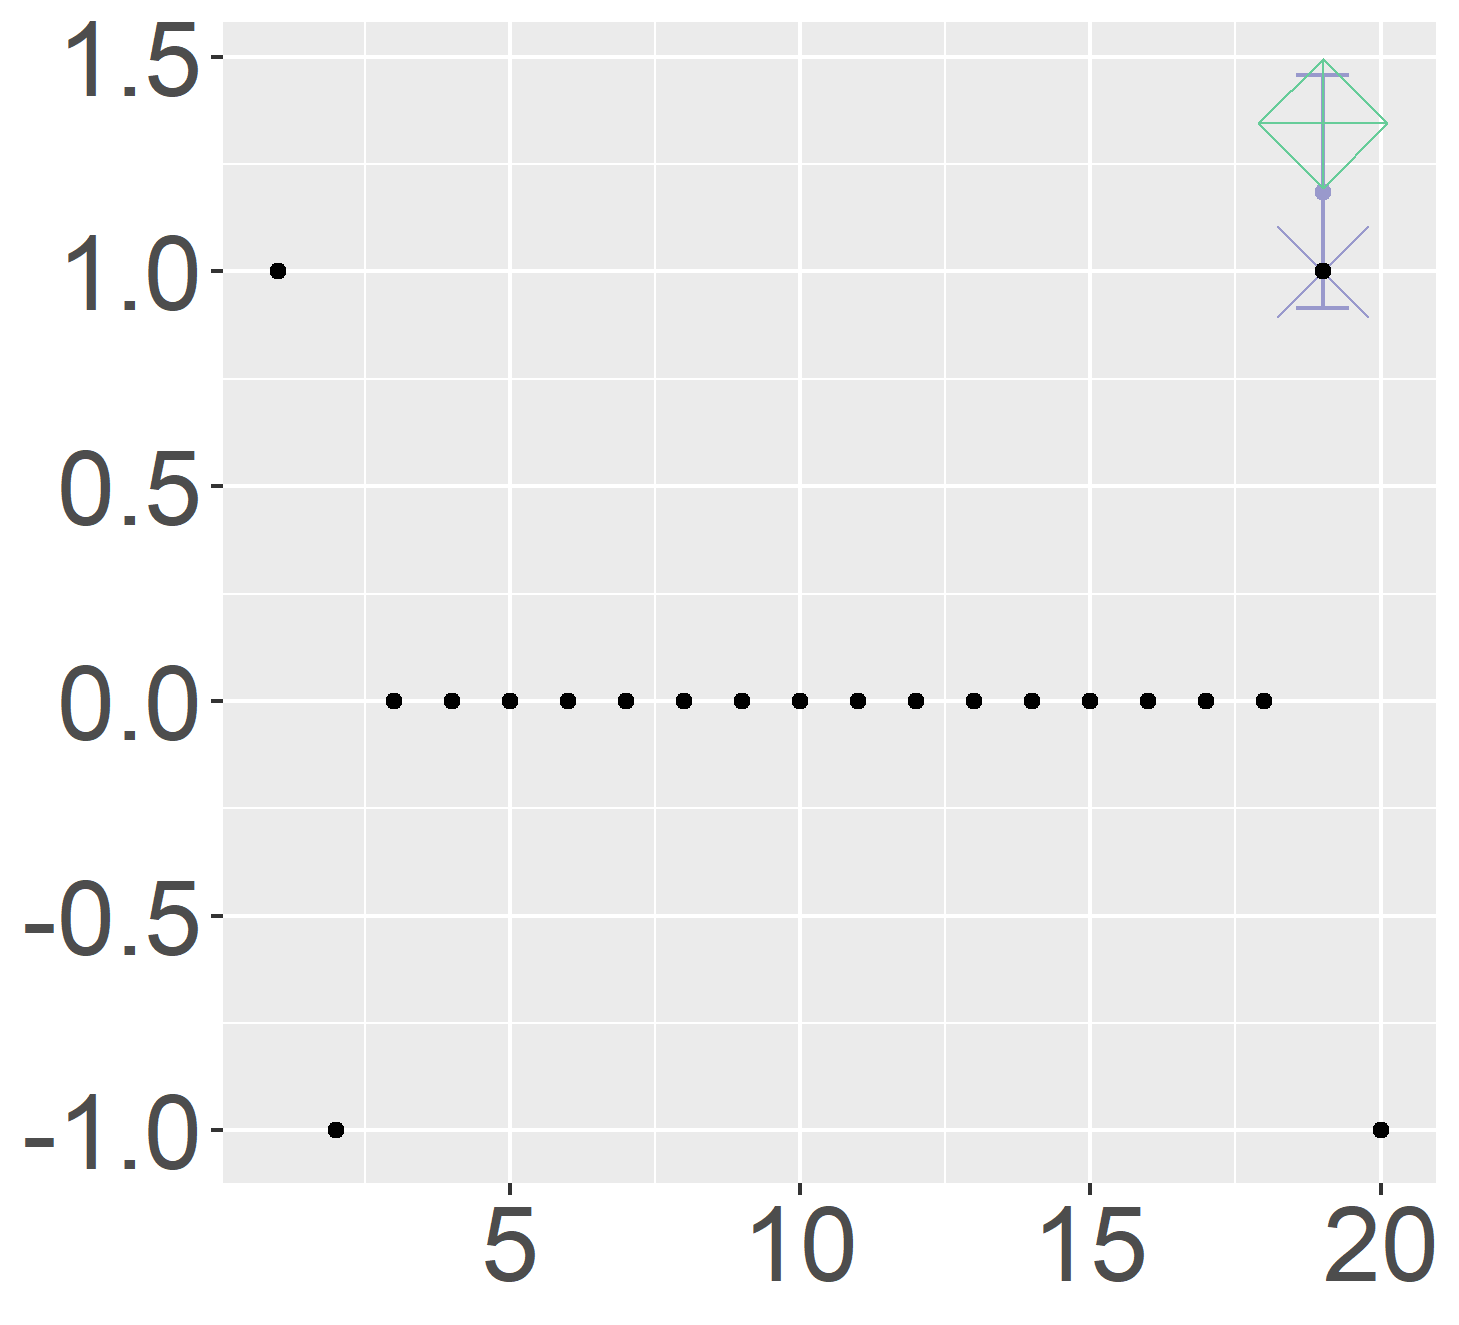
\includegraphics[width=\columnwidth]{../../plot/p2_10_1_1.png}
    \caption{(c) Data fission (P2) $n=10$}
\end{subfigure}
\\
\centering
\begin{subfigure}[b]{.32\columnwidth} 
    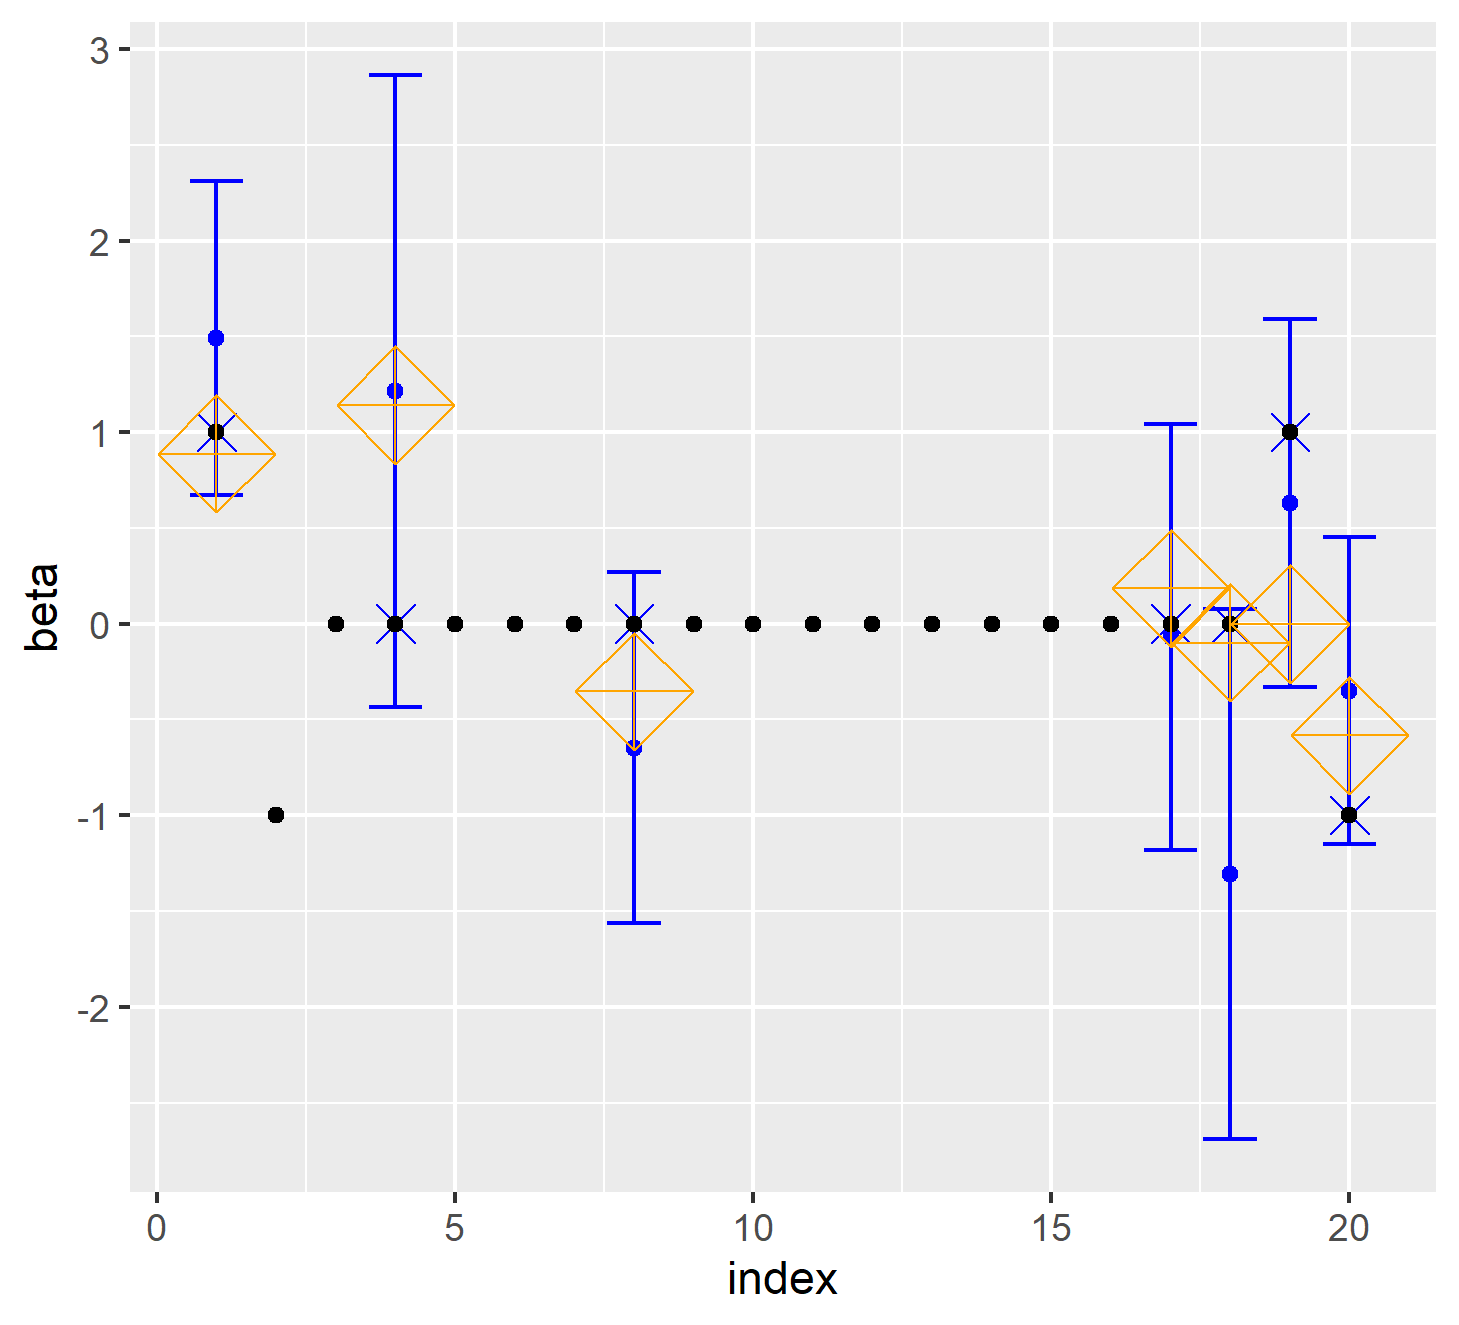
\includegraphics[width=\columnwidth]{../../plot/split_20_1_1.png}
    \caption{(d) Data splitting $n=20$}
\end{subfigure}
\hfill
\centering
\begin{subfigure}[b]{.32\columnwidth} 
    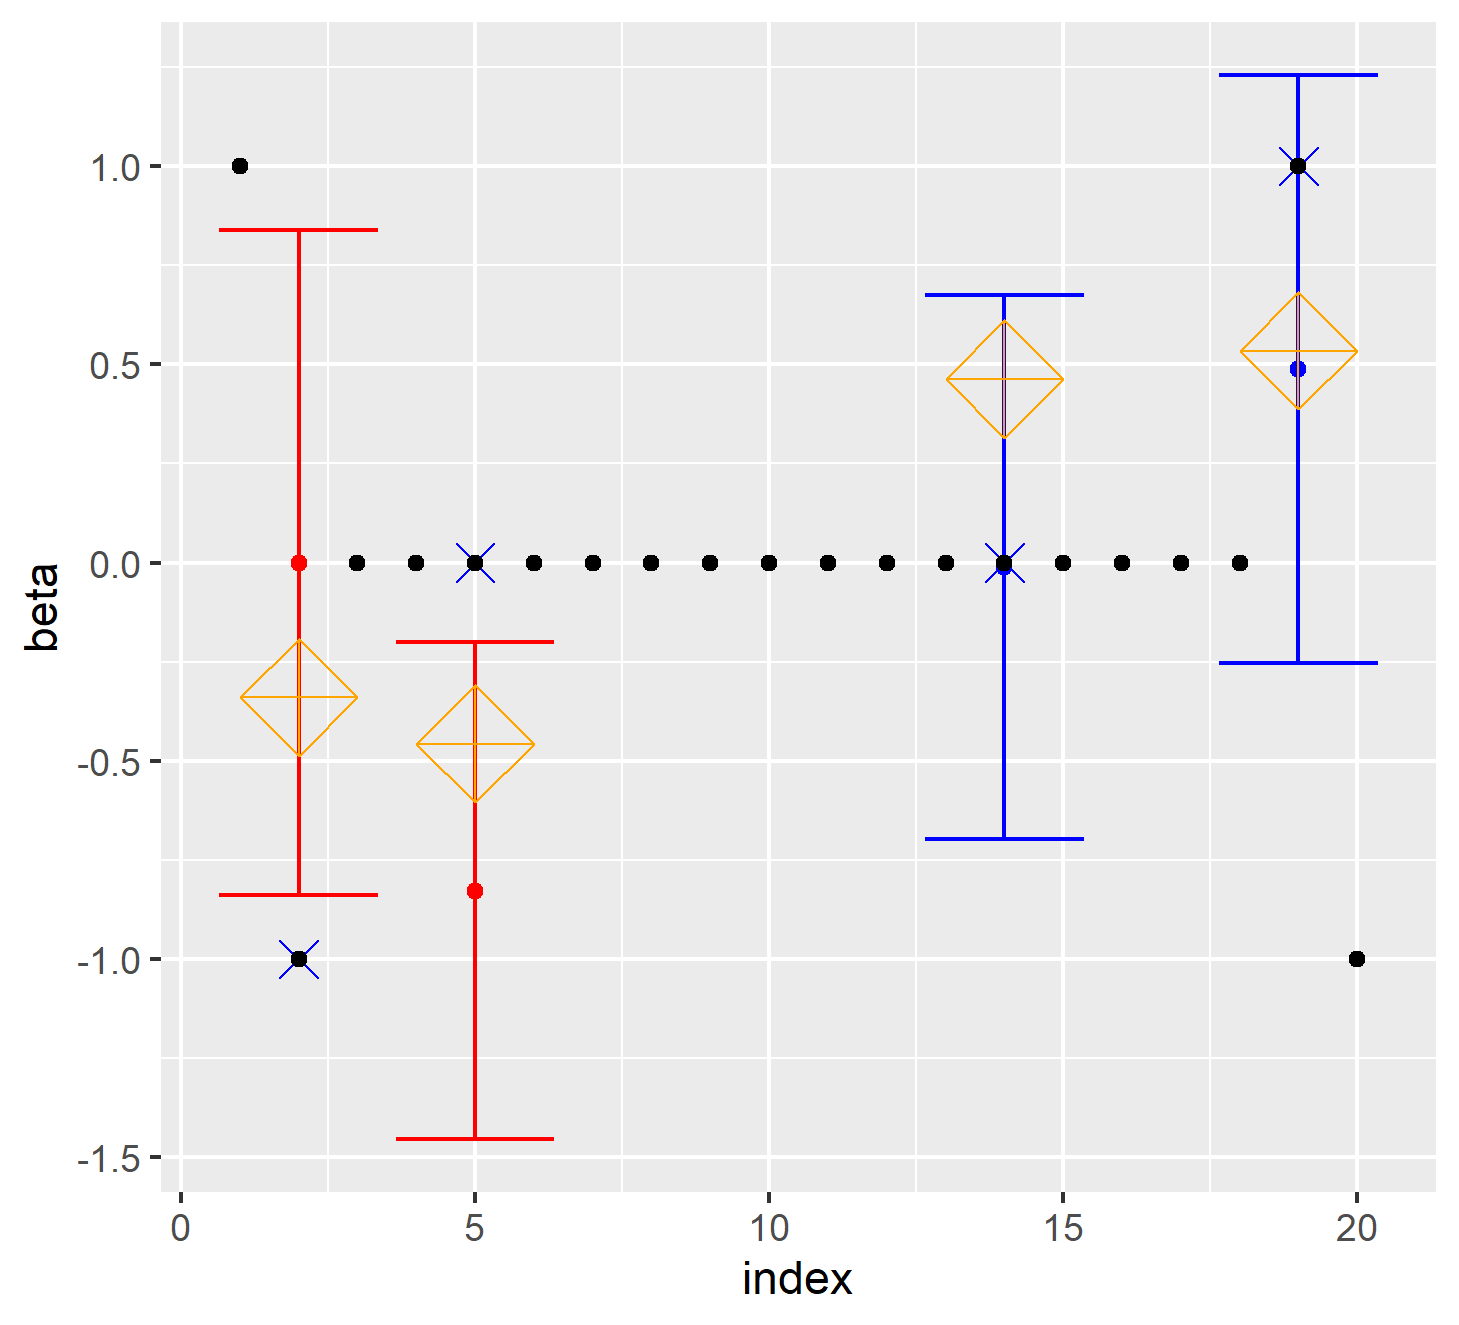
\includegraphics[width=\columnwidth]{../../plot/p1_20_1_1.png}
    \caption{(e) Data fission (P1) $n=20$}
\end{subfigure}
\hfill
\centering
\begin{subfigure}[b]{.32\columnwidth} 
    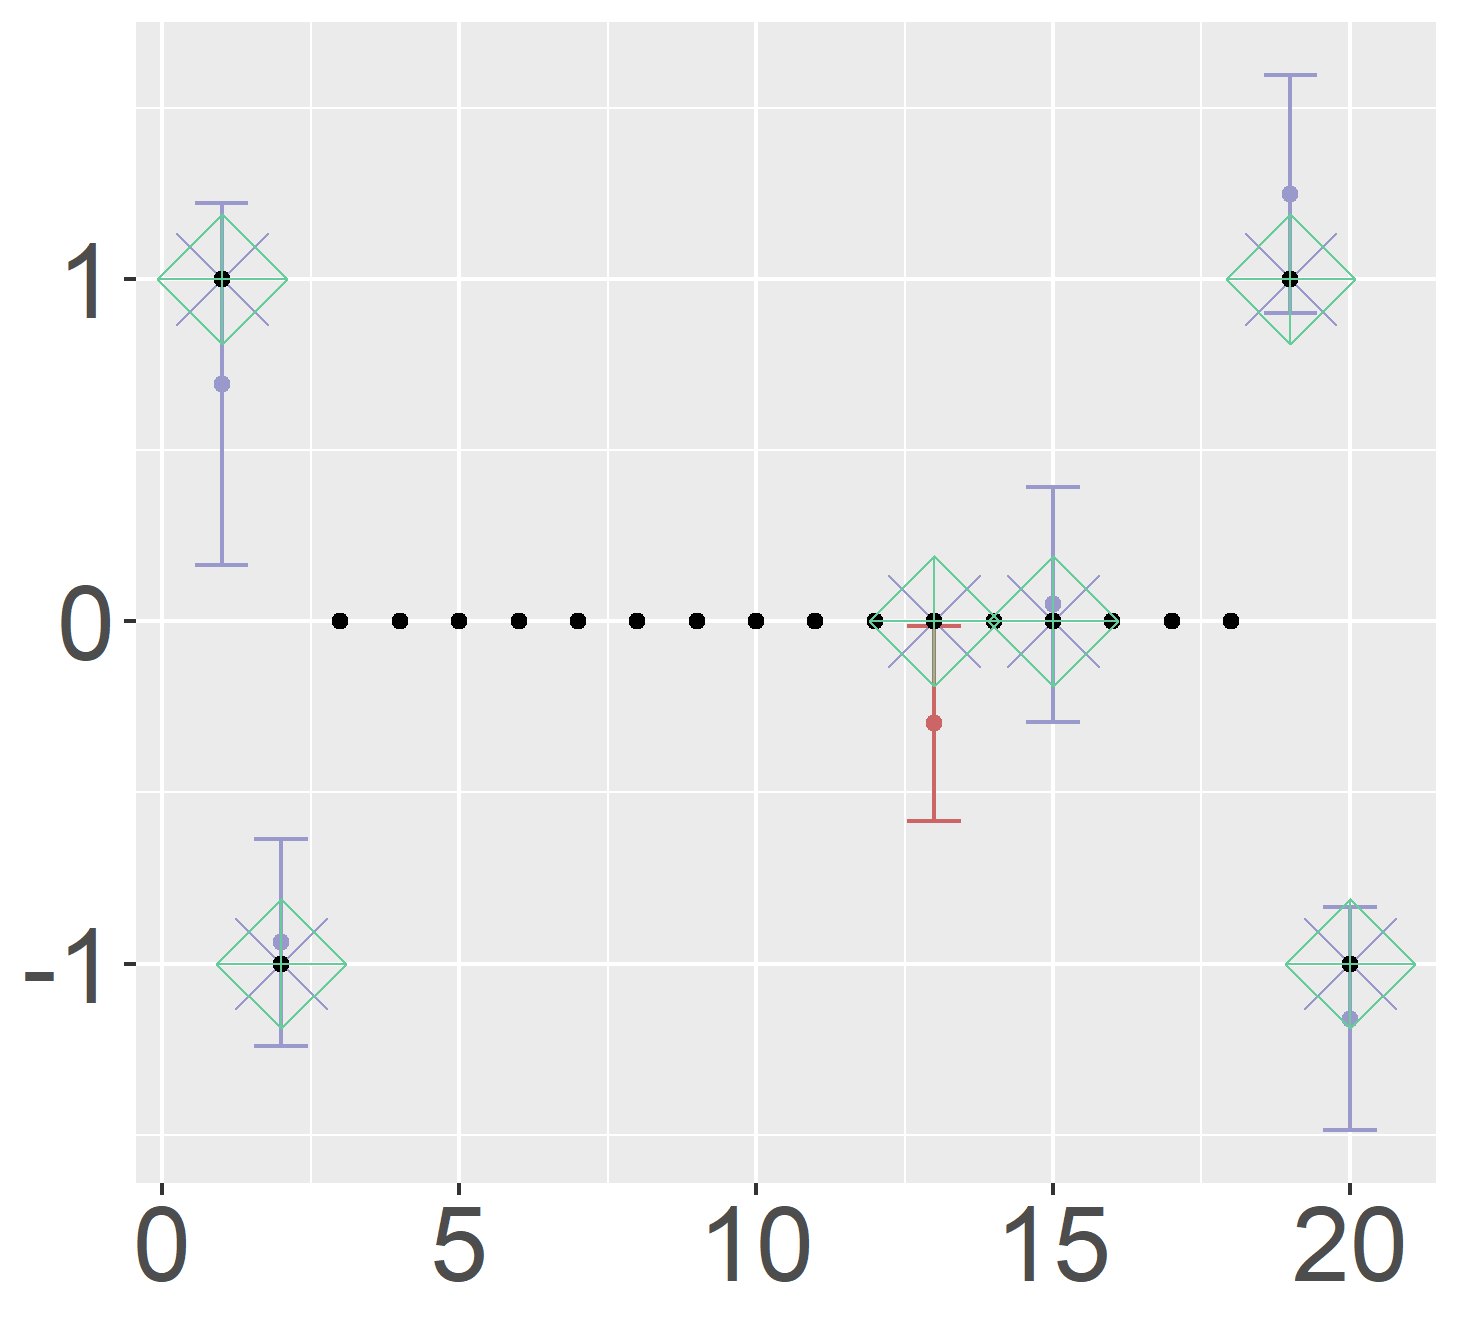
\includegraphics[width=\columnwidth]{../../plot/p2_20_1_1.png}
    \caption{(f) Data fission (P2) $n=20$}
\end{subfigure}
\\
\centering
\begin{subfigure}[b]{.32\columnwidth} 
    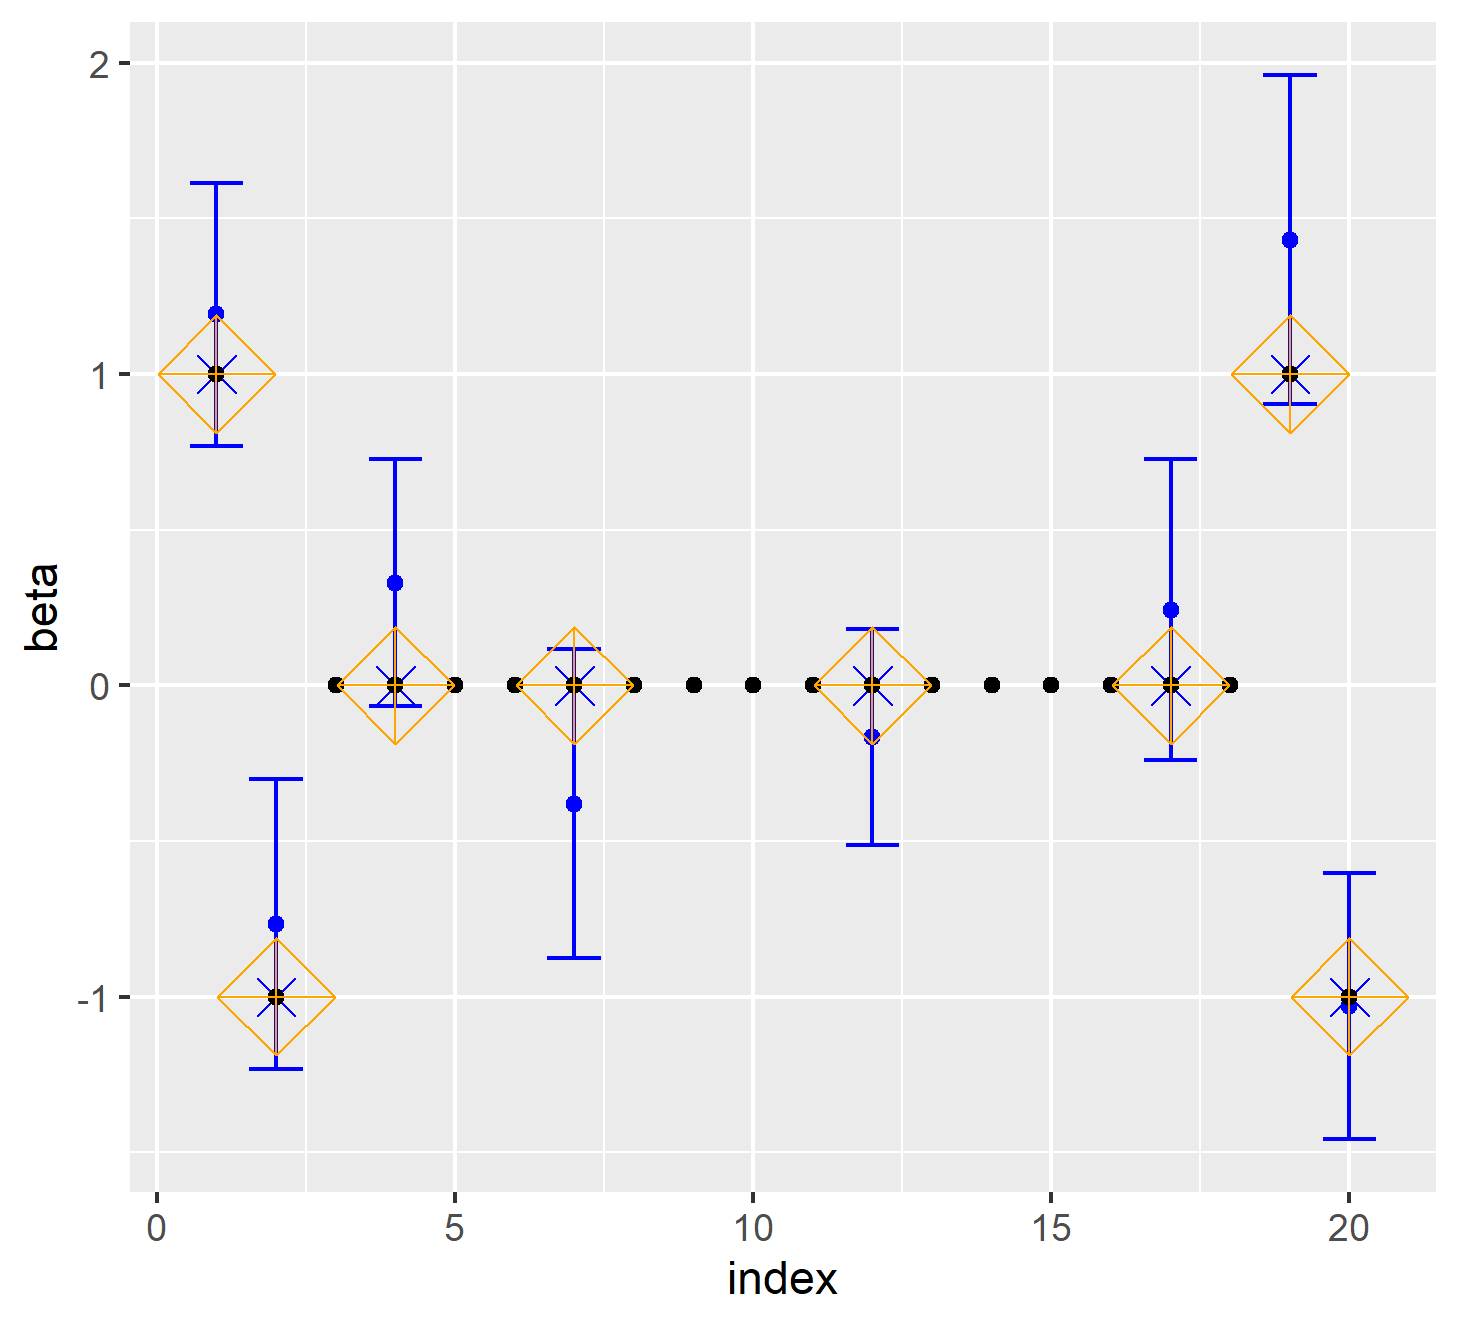
\includegraphics[width=\columnwidth]{../../plot/split_50_1_1.png}
    \caption{(g) Data splitting $n=50$}
\end{subfigure}
\hfill
\centering
\begin{subfigure}[b]{.32\columnwidth} 
    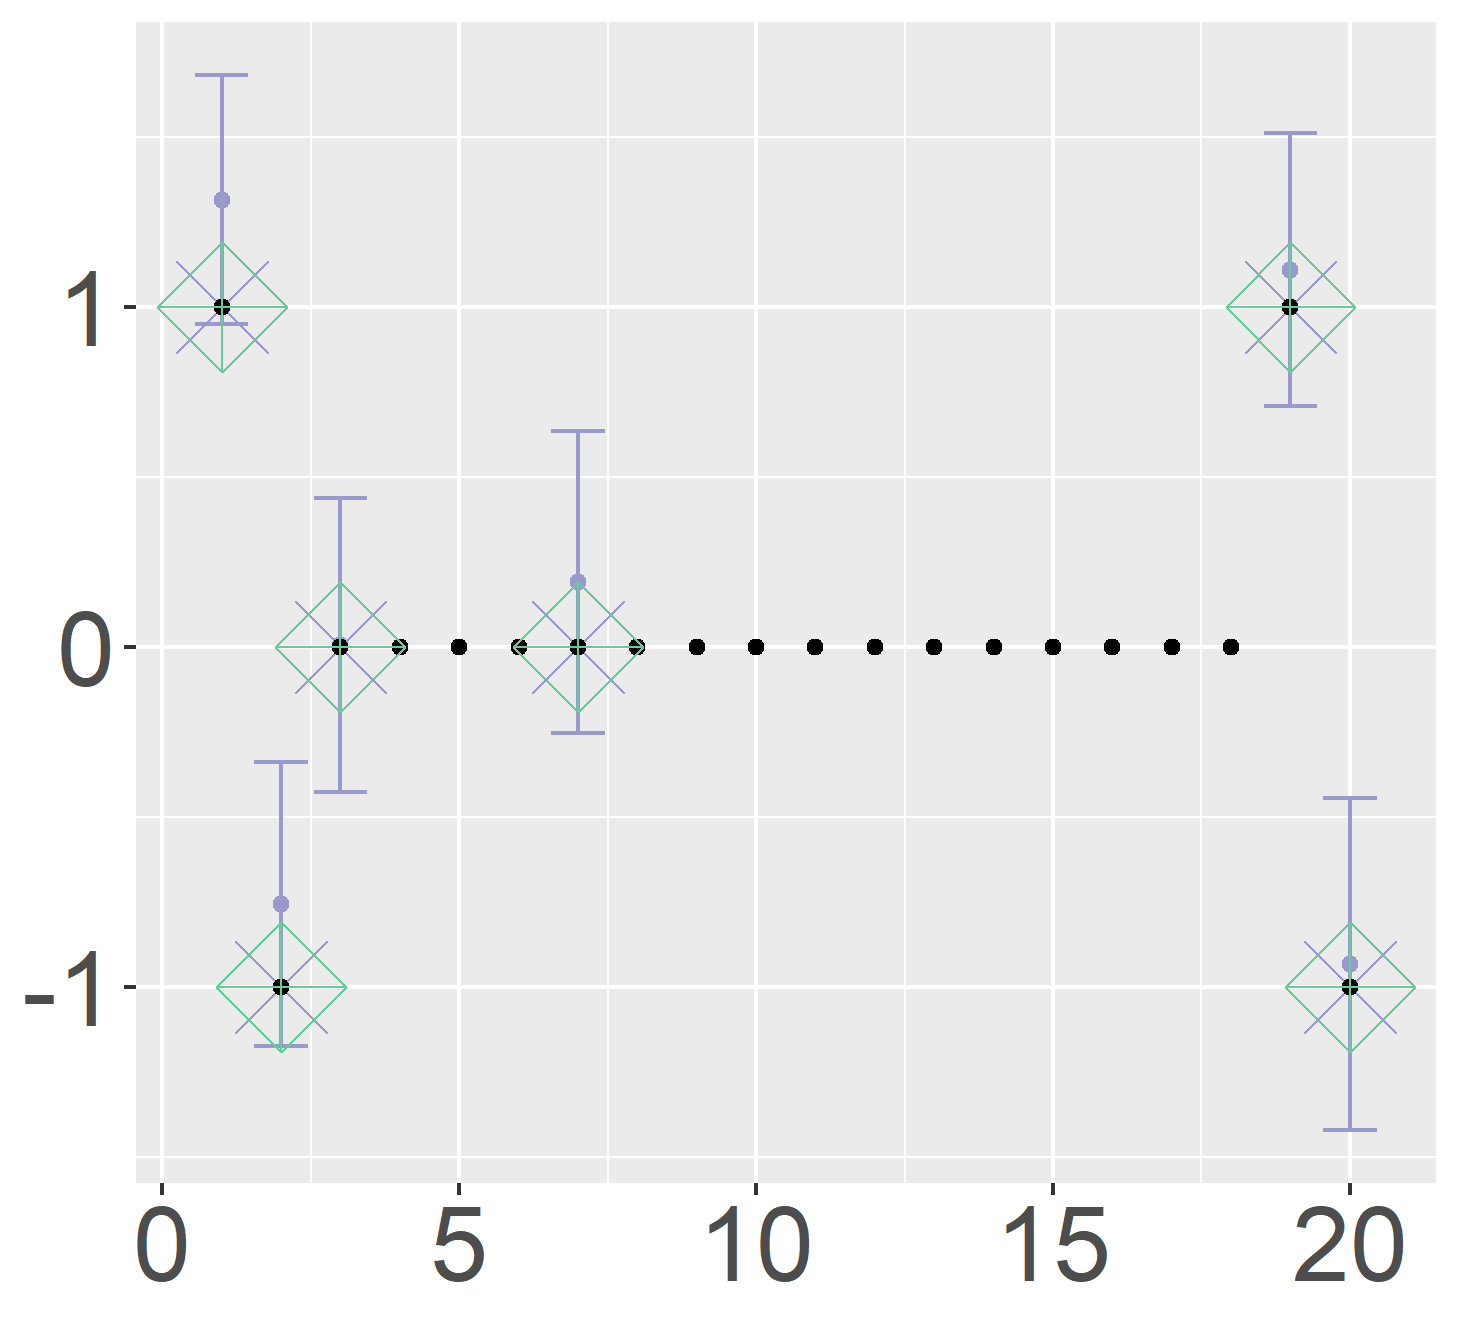
\includegraphics[width=\columnwidth]{../../plot/p1_50_1_1.png}
    \caption{(h) Data fission (P1) $n=50$}
\end{subfigure}
\hfill
\centering
\begin{subfigure}[b]{.32\columnwidth} 
    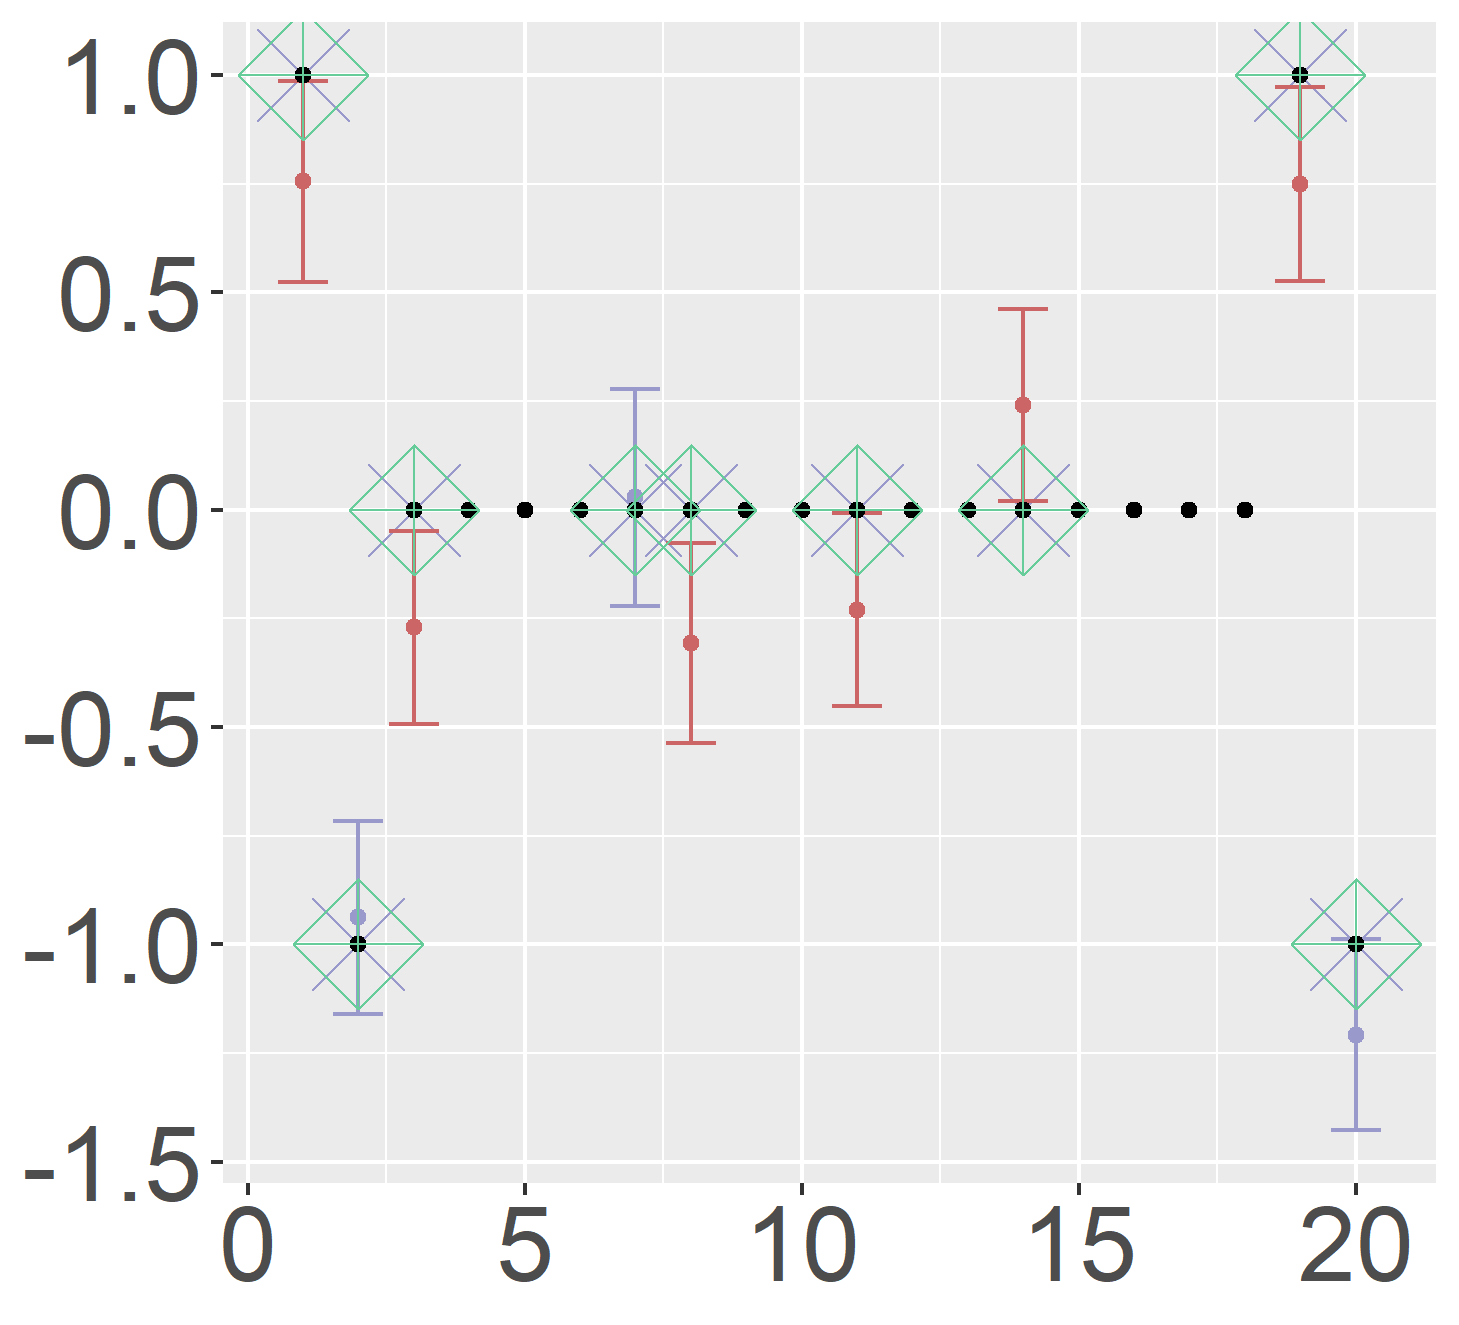
\includegraphics[width=\columnwidth]{../../plot/p2_50_1_1.png}
    \caption{(i) Data fission (P2) $n=50$}
\end{subfigure}
\\
\centering
\begin{subfigure}[b]{.32\columnwidth} 
    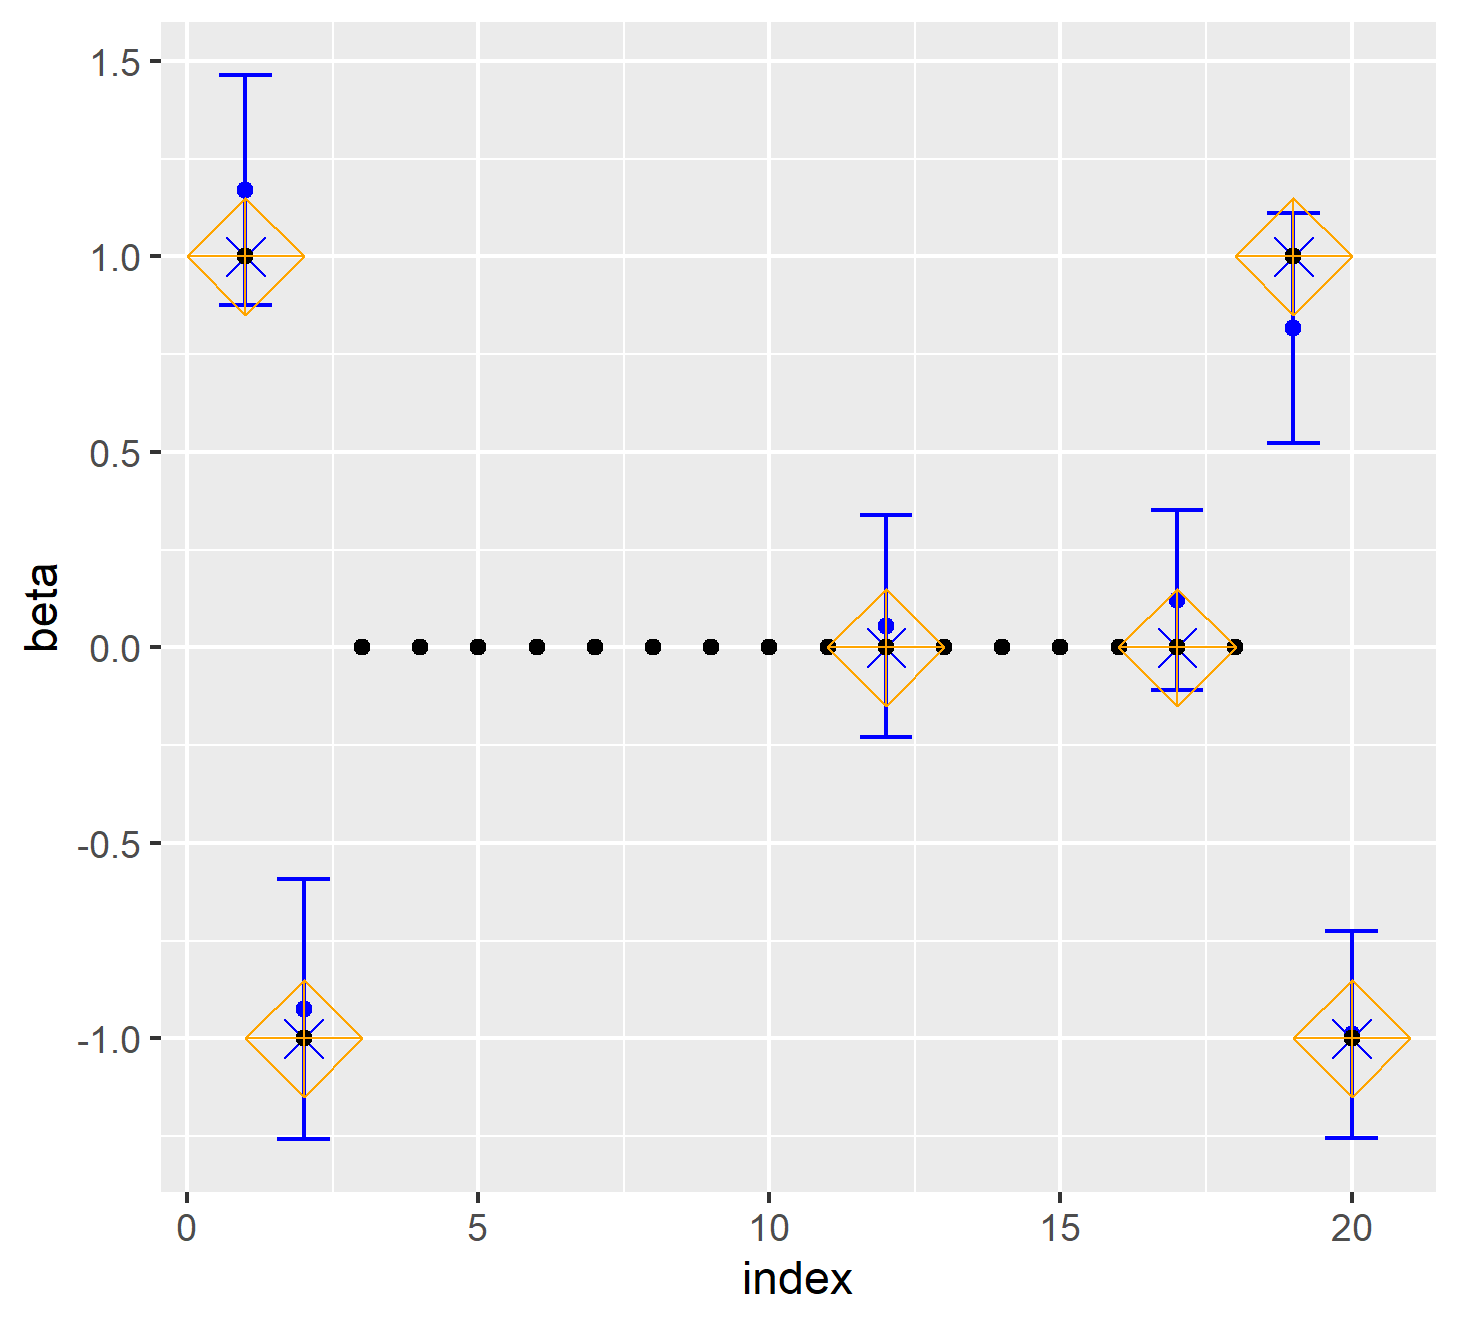
\includegraphics[width=\columnwidth]{../../plot/split_100_1_1.png}
    \caption{(j) Data splitting $n=100$}
\end{subfigure}
\hfill
\centering
\begin{subfigure}[b]{.32\columnwidth} 
    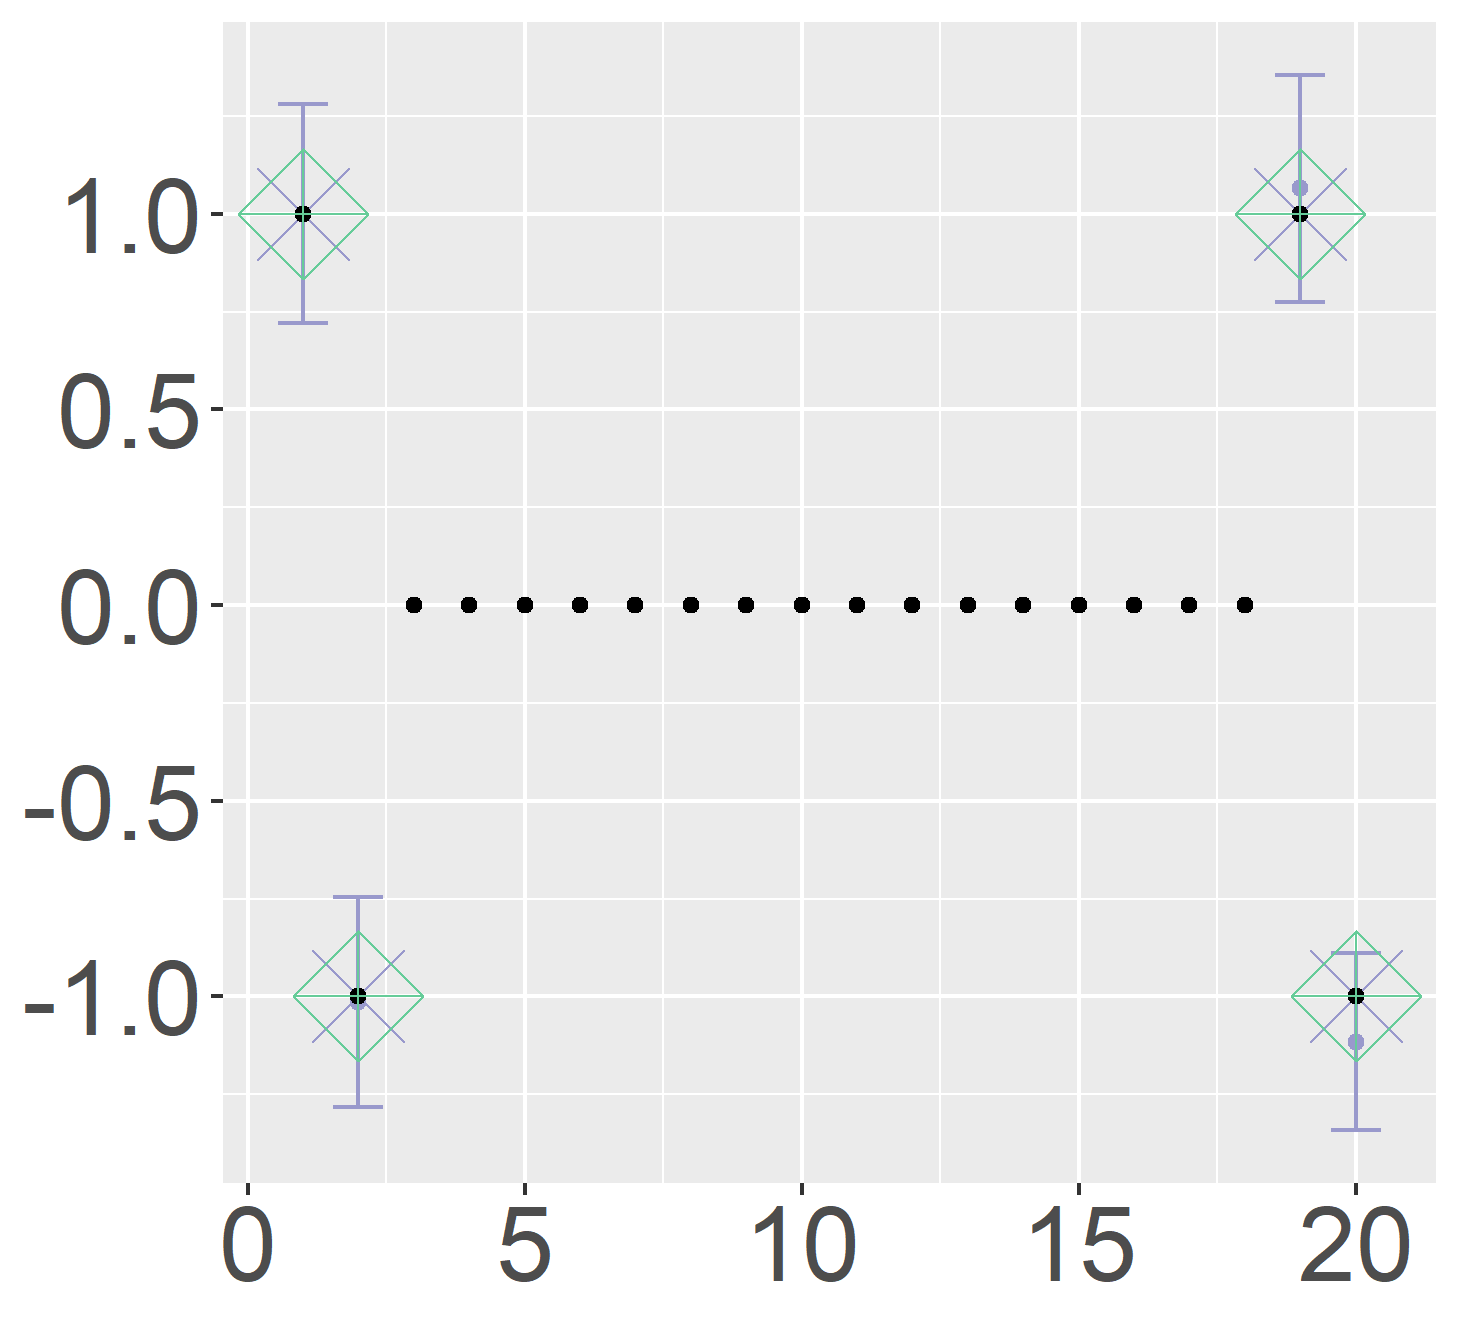
\includegraphics[width=\columnwidth]{../../plot/p1_100_1_1.png}
    \caption{(k) Data fission (P1) $n=100$}
\end{subfigure}
\hfill
\centering
\begin{subfigure}[b]{.32\columnwidth} 
    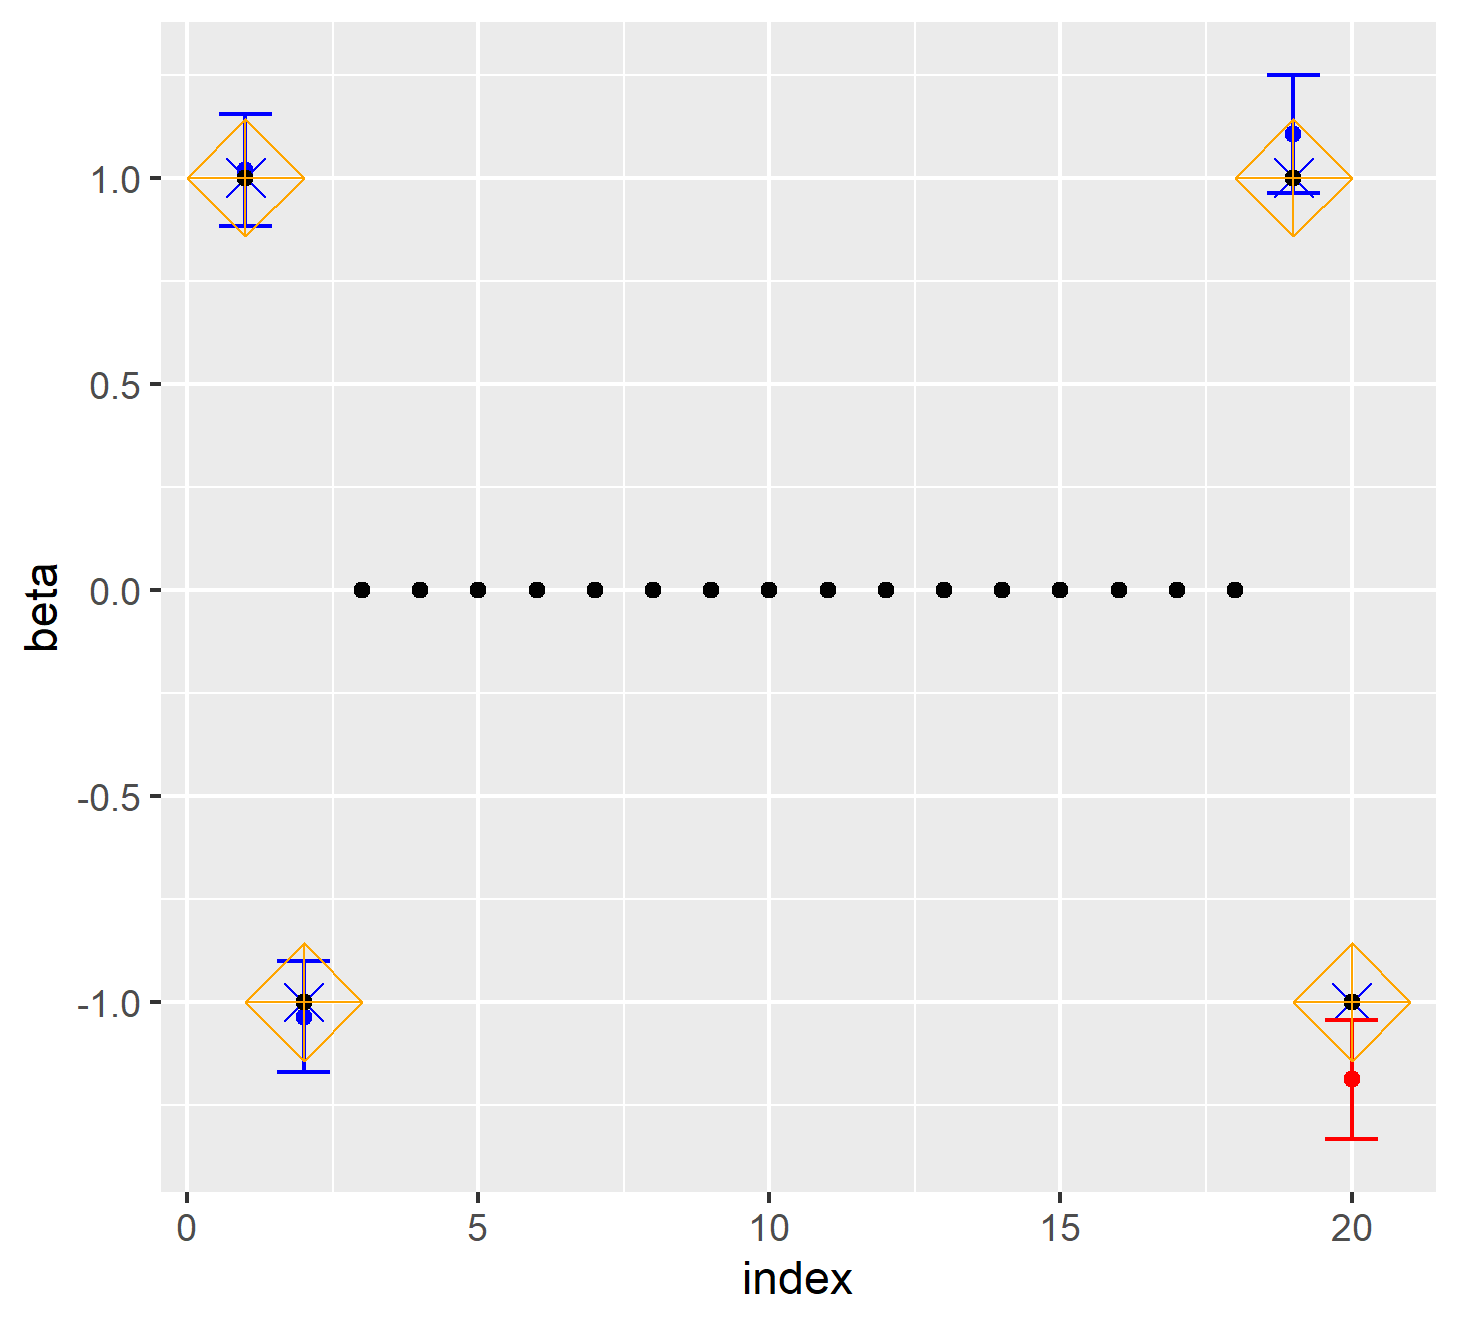
\includegraphics[width=\columnwidth]{../../plot/p2_100_1_1.png}
    \caption{(l) Data fission (P2) $n=100$}
    \label{fig:p2_100}
\end{subfigure}
\caption{introduce legend and what coverage color means}
\label{fig:individual}
\end{figure}